 %TCIDATA{Version=5.00.0.2557}
%TCIDATA{LaTeXparent=0,0,dissosw.tex}

%TCIDATA{ChildDefaults=chapter:2,page:1}

%comecei a trabalhar na versao final em 15 de junho de 2009

\chapter{Física de Partículas e o detector ATLAS}

Os experimentos de Física de Partículas Elementares têm como
principais objetivos a confirmação de modelos desenvolvidos
teoricamente e a identificação de novos fenômenos. O experimento
LHC~\cite{article:LHC:2008} é o maior acelerador de partículas já
desenvolvido e quando operando em máxima capacidade, serão gerados
aproximadamente $10^9$ interações por segundo. Os detectores são
responsáveis por selecionar, dentro de um conjunto enorme, os
eventos de real interesse, que são bastante raros. O projeto e a
montagem do detector ATLAS (\textit{A Thoroidal LHC Apparatus})
\cite{article:ATLAS:2008} foram conduzidos por uma cola\-bo\-ração
de 36 países, conhecida como \textit{ATLAS Collaboration}, contando
com pesquisadores de mais de 150 universidades e centros de
pesquisa~\cite{Homepage:ATLAS}. Sendo um dos detectores de propósito
geral do experimento LHC, o ATLAS tem formato cilíndrico e foi
projetado para cobrir um ângulo sólido próximo a $4\pi$ ao redor da
região de colisão.


\section{Panorama geral da física de partículas elementares}

A noção de que a matéria é composta por um conjunto de constituintes
elementares existe há mais de 2000 anos, desde o tempo dos filósofos
gregos~\cite{book:fernow:1986}. No decorrer do século 20, a
compreensão dos componentes elementares da matéria forneceu à
comunidade científica mundial informações importantes a res\-peito
das leis fundamentais da natureza. O estudo da física de partículas
elementares teve início no final do século 19, quando foi descoberto
o elétron, experimentando um crescimento acen\-tua\-do na década de
1950, quando foram descobertas centenas de novas partículas. A partir de sua criação 
em 1954, o CERN (Centro Europeu para Pesquisa Nuclear) contribuiu significativamente
nesse processo.

Inicialmente, pensava-se que a matéria era constituída de partículas
subatô\-micas, chamadas elétrons, prótons e nêutrons. Mais tarde,
descobriu-se que os prótons e nêutrons são compostos de quarks. Hoje
sabe-se que toda a matéria no universo é composta de léptons e
quarks. Existem ainda outras partículas elementares que são
responsáveis por promover a interação entre léptons e quarks.
Juntamente com as descobertas experimentais, estudos teóricos
possibilitaram o desenvolvimento do Modelo Padrão
(SM-\textit{Standard Model})~\cite{livro:fisica1:2006} que descreve
e prevê, de forma unificada, o comportamento das partículas e das
forças de interação.

As características e propriedades dos processos nucleares dependem
da ener\-gia envolvida. A unidade de energia mais utilizada,
neste contexto, é o elétron-volt (eV) e seus múltiplos (MeV, GeV ou
TeV). O elétron-volt é definido como a energia necessária para
aumentar o potencial elétrico de um elétron em 1 volt (em unidades
do Sistema Internacional - SI temos: 1eV$=$1,6$\times
10^{-19}$J)~\cite{book:martin:2006}. Os fenômenos produzidos quando
a energia das partículas é menor que $20MeV$ são chamados de física
a baixas energias. A faixa entre $20MeV$ e $400MeV$ corresponde à
física a energias intermediárias, e finalmente, fenômenos com
energia superior a $400MeV$ são estudados na física a altas
energias~\cite{book:chung:2001}.

%, extraído de \cite{livro:fisica1:2006}

Os experimentos realizados a partir do início da década de 1970
foram fundamentais para o desenvolvimento e teste do Modelo Padrão,
mas também despertaram dúvidas a respeito de questões que não são
completamente respondidas. O SM (ver Figura \ref{SM}), divide as
partículas elementares em quarks e léptons. Existem seis tipos de
léptons (elétron, múon, tau e três neutrino) e seis tipos de quarks
(\textit{up}, \textit{down}, \textit{charm}, \textit{strange},
\textit{top} e \textit{bottom}).

\begin{figure}[h!] \centering
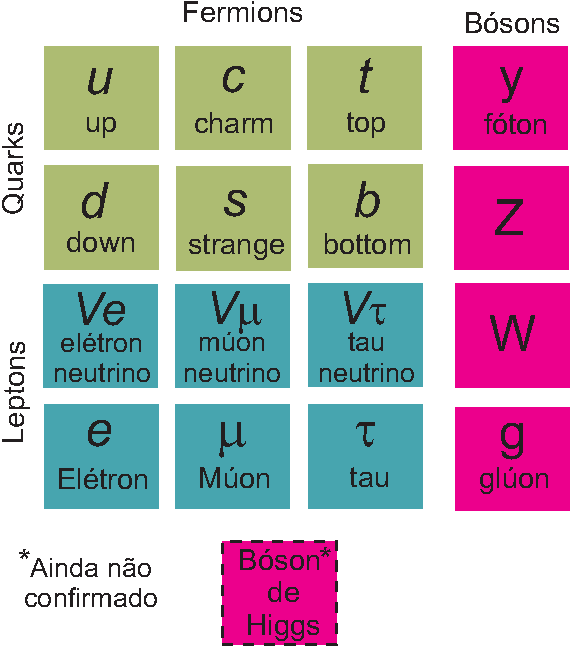
\includegraphics[width=7cm]{cap2_sm}
\caption{Diagrama do Modelo Padrão, mostrando as partículas
elementares incluindo o, ainda não confirmado, bóson de Higgs.}
\label{SM}
\end{figure}

Atualmente são conhecidas quatro formas de interação (ou
acoplamento) entre as partículas elementares, são elas
eletromagnética, gravitacional, fraca e forte. A força gravitacional
é predominante entre corpos massivos separados por longas
distâncias. Entre partículas, onde a massa é da ordem de
$10^{-27}$Kg, a interação gravitacional tem intensidade muito baixa.
Para distâncias maiores que $10^{-13}$cm, a força eletromagnética
domina, enquanto que para distancias menores, as interações forte e
fraca se destacam. A intensidade relativa (em comparação com a interação forte) dos quatro tipos de
interação é mostrada na Tabela \ref{tab_forcas}
\cite{book:mist:2003}.

\begin{table}[b!]
\centering
\begin{tabular}{cc }
  \hline
  % after \\: \hline or \cline{col1-col2} \cline{col3-col4} ...
  \textbf{Interação} & \textbf{Intensidade Relativa} \\  \hline
  Forte  &  1 \\
  Eletromagnética  & $10^{-2}$\\
  Fraca & $10^{-5}$ \\
  Gravitacional & $10^{-39}$ \\
  \hline
\end{tabular}
\caption{Intensidade relativa (em comparação com a interação forte) dos diversos tipos de interação.}
\label{tab_forcas}
\end{table}

Existem algumas teorias que descrevem como as interações elementares
ocorrem. A eletrodinâmica quântica (QED - \textit{Quantum
Eletrodynamics}) considera que os processos elétricos e magnéticos
acontecem a partir da interação fundamental entre dois elétrons, com
a troca de um fóton. O fóton é a partícula mediadora da interação
eletromagnética.

De modo semelhantes são definidos os outros tipos de interação. Para
a interação forte, as partículas mediadoras são os glúons. Os bósons
W e Z mediam a interação fraca e o gráviton a interação
gravitacional. A teoria da cromodinâmica quântica (QCD -
\textit{Quantum Chromodynamics}) \cite{book:QCD:2003}, por exemplo,
descreve como os quarks e glúons interagem para formar os hadrons
(prótons e neutrons são exem\-plos de hádrons). Uma diferença entre
a QED e a QCD é que na última, os quarks e glúons não são observados
como partículas livres (mas apenas na forma de hádrons), em oposição
aos elétrons e fótons da QED. Mesmo em colisões de alta energia,
quando quarks são produzidos, eles se afastam rapidamente uns dos
outros, e antes que possam ser observados, se convertem em ``jatos"
de hádrons (ou jatos hadrônicos)~\cite{book:martin:2006}.

Considerando uma teoria atualmente aceita pela física teórica
(conhecida como \textit{Gauge Invariance}) e as partículas e formas
de interação já verificadas experimentalmente, todas as partículas
elementares teriam massa nula. Esta previsão é contrária aos
resultados experimentais e somente pode ser corrigida assumindo-se
que existe um outro tipo de interação. Esta interação foi prevista
pelo cientista inglês Peter Higgs em 1964, tendo como partícula
mediadora o bóson de Higgs, que é responsável por fornecer massa às
partículas~\cite{book:martin:2006}. A existência do bóson de Higgs é
a mais importante previsão do modelo padrão ainda não verificada
experimentalmente e sua busca é de máxima importância para a física
de partículas.

Nas últimas décadas, os experimentos com aceleradores de partículas
se tornaram gigantescos empreendimentos envolvendo milhares de
físicos e engenheiros com contribuição financeira e intelectual de
dezenas de países. Os aceleradores usam força eletromagnética para
aumentar a energia de partículas estáveis e carregadas
eletricamente. As partículas são injetadas na máquina por
dispositivos que produzem uma fonte de partículas de alta
intensidade e baixa energia. Quanto às características construtivas,
os aceleradores podem ser divididos em alvo-fixo ou colisionadores
de feixes. Nos aceleradores de alvo-fixo, as partículas são
aceleradas até a máxima energia, quando o feixe é retirado da
máquina e direcionado a um alvo estacionário. Nos colisionadores,
feixes de partículas são acelerados e quando a energia desejada é
atingida, os feixes são colocados em rota de colisão em alguns
pontos específicos do percurso. Quanto ao percurso dos feixes, os
aceleradores podem ser lineares ou circulares \cite{book:martin:2006}.

Imediatamente após a colisão, uma grande quantidade de partículas
elementares é produzida. Algumas delas são estáveis, porém outras
têm curtíssimo tempo de vida. Os elétrons e prótons, por exemplo,
têm vida média superior a $10^{23}$ anos, enquanto os múons podem
ter vida média da ordem de $10^{-6}$ segundos
\cite{book:chung:2001}. Para que todos os eventos sejam corretamente
identificados, um complexo sistema de detecção precisa ser
construído.

A massa (m) das partículas é usualmente expressa em função da
energia equi\-va\-lente ($m=E/c^2$, onde $c$ é a velocidade da luz e
$E$ a energia). Os bósons W e Z, por exemplo, têm massa de 80 e 91
GeV/c$^2$ (onde 1GeV/c$^2$=1,78$\times 10^{-27}$ kg). Na Tabela
\ref{tab_massa}, são mostradas as massas de algumas partículas
importantes. Ainda não é possível determinar a massa esperada para o
bóson de Higgs, porém, considerando o conhe\-ci\-men\-to adquirido
com os experimentos operados antes do LHC, sua massa deve ser
maior que 115 GeV/c$^2$ \cite{livro:fisica1:2006}.

O acelerador LHC (\textit{Large Hadron Collider} - Grande
Colisionador Hadrônico)~\cite{article:LHC:2008,article:LHC:2002} em
operação no CERN (Centro Europeu para Pesquisa Nuclear)
\cite{Homepage:CERN}, será capaz de atingir energia de até 14 TeV e
permitir à visualização do bóson de Higgs, caso o Modelo Padrão
esteja correto.

\begin{table}[h!]
\centering
\begin{tabular}{cc }
  \hline
  % after \\: \hline or \cline{col1-col2} \cline{col3-col4} ...
  \textbf{Partícula} & \textbf{Massa (GeV/c$^2$)} \\  \hline
  Elétron  &  0,000511 \\
  Próton  & 0,938 \\
  Bóson W & 80 \\
  Bóson Z & 91 \\
  Bóson de Higgs ou outras novas partículas & $>$115 \\
  \hline
\end{tabular}
\caption{Exemplos de valores da massa (em energia equivalente) de
algumas partículas.} \label{tab_massa}
\end{table}

Além da busca pelo bóson de Higgs, existem outras questões que
precisam ser respondidas em física de partículas. É um desejo antigo dos físicos, desde
Einstein, a unificação das teorias sobre as forças entre as
partículas, incluindo no Modelo Padrão a força gravitacional. O
estudo da física de partículas também é fundamental para o
entendimento da natureza e origem do universo. Pretende-se, por
exemplo, descobrir informações sobre a composição da matéria escura
\cite{article:darkm:2005}, super-simetria \cite{article:susy:1996} e
violação de CP (do inglês \textit{Charge
Parity})~\cite{book:cpv:1999}.

Entre os laboratórios que conduzem experimentos em física de
partículas os principais são: CERN, DESY \cite{Homepage:desy}, KEK
\cite{homepage:kek}, Fermilab \cite{Homepage:Fermilab}, SLAC
\cite{homepage:slac} e Brookhaven \cite{Homepage:brookhaven},
localizados respectivamente na Suíça, Alemanha, Japão e os três
últimos nos Estados Unidos.
%citar as homepages dos laboratórios

O CERN, fundado em 1954, é atualmente um dos maiores centros de
pesquisas em física de partículas do mundo. Localizado em Genebra,
Suíça, funciona com base num complexo sistema de colaboração
internacional, que envolve centenas de instituições de pesquisa em
centenas de paises \cite{Homepage:CERN}.

\section{O acelerador LHC}

No CERN, foi projetado e construído o experimento LHC (\textit{Large
Hadron Collider}), que iniciou sua operação no final de 2008
\cite{article:LHC:2008,Homepage:lhc}. O LHC pode atingir níveis de
energia de, aproximadamente, \linebreak 14 TeV. O percurso do
acelerador, localizado na fronteira franco-suíça, é aproximadamente
circular, com 27 Km de comprimento, numa profundidade do solo que
varia de 50 a 150 metros (ver Figura \ref{mapaLHC}). Feixes de
prótons serão acelerados em sentidos opostos e direcionados para
colisão nos centros dos detectores.

\begin{figure}[b!]
\centering
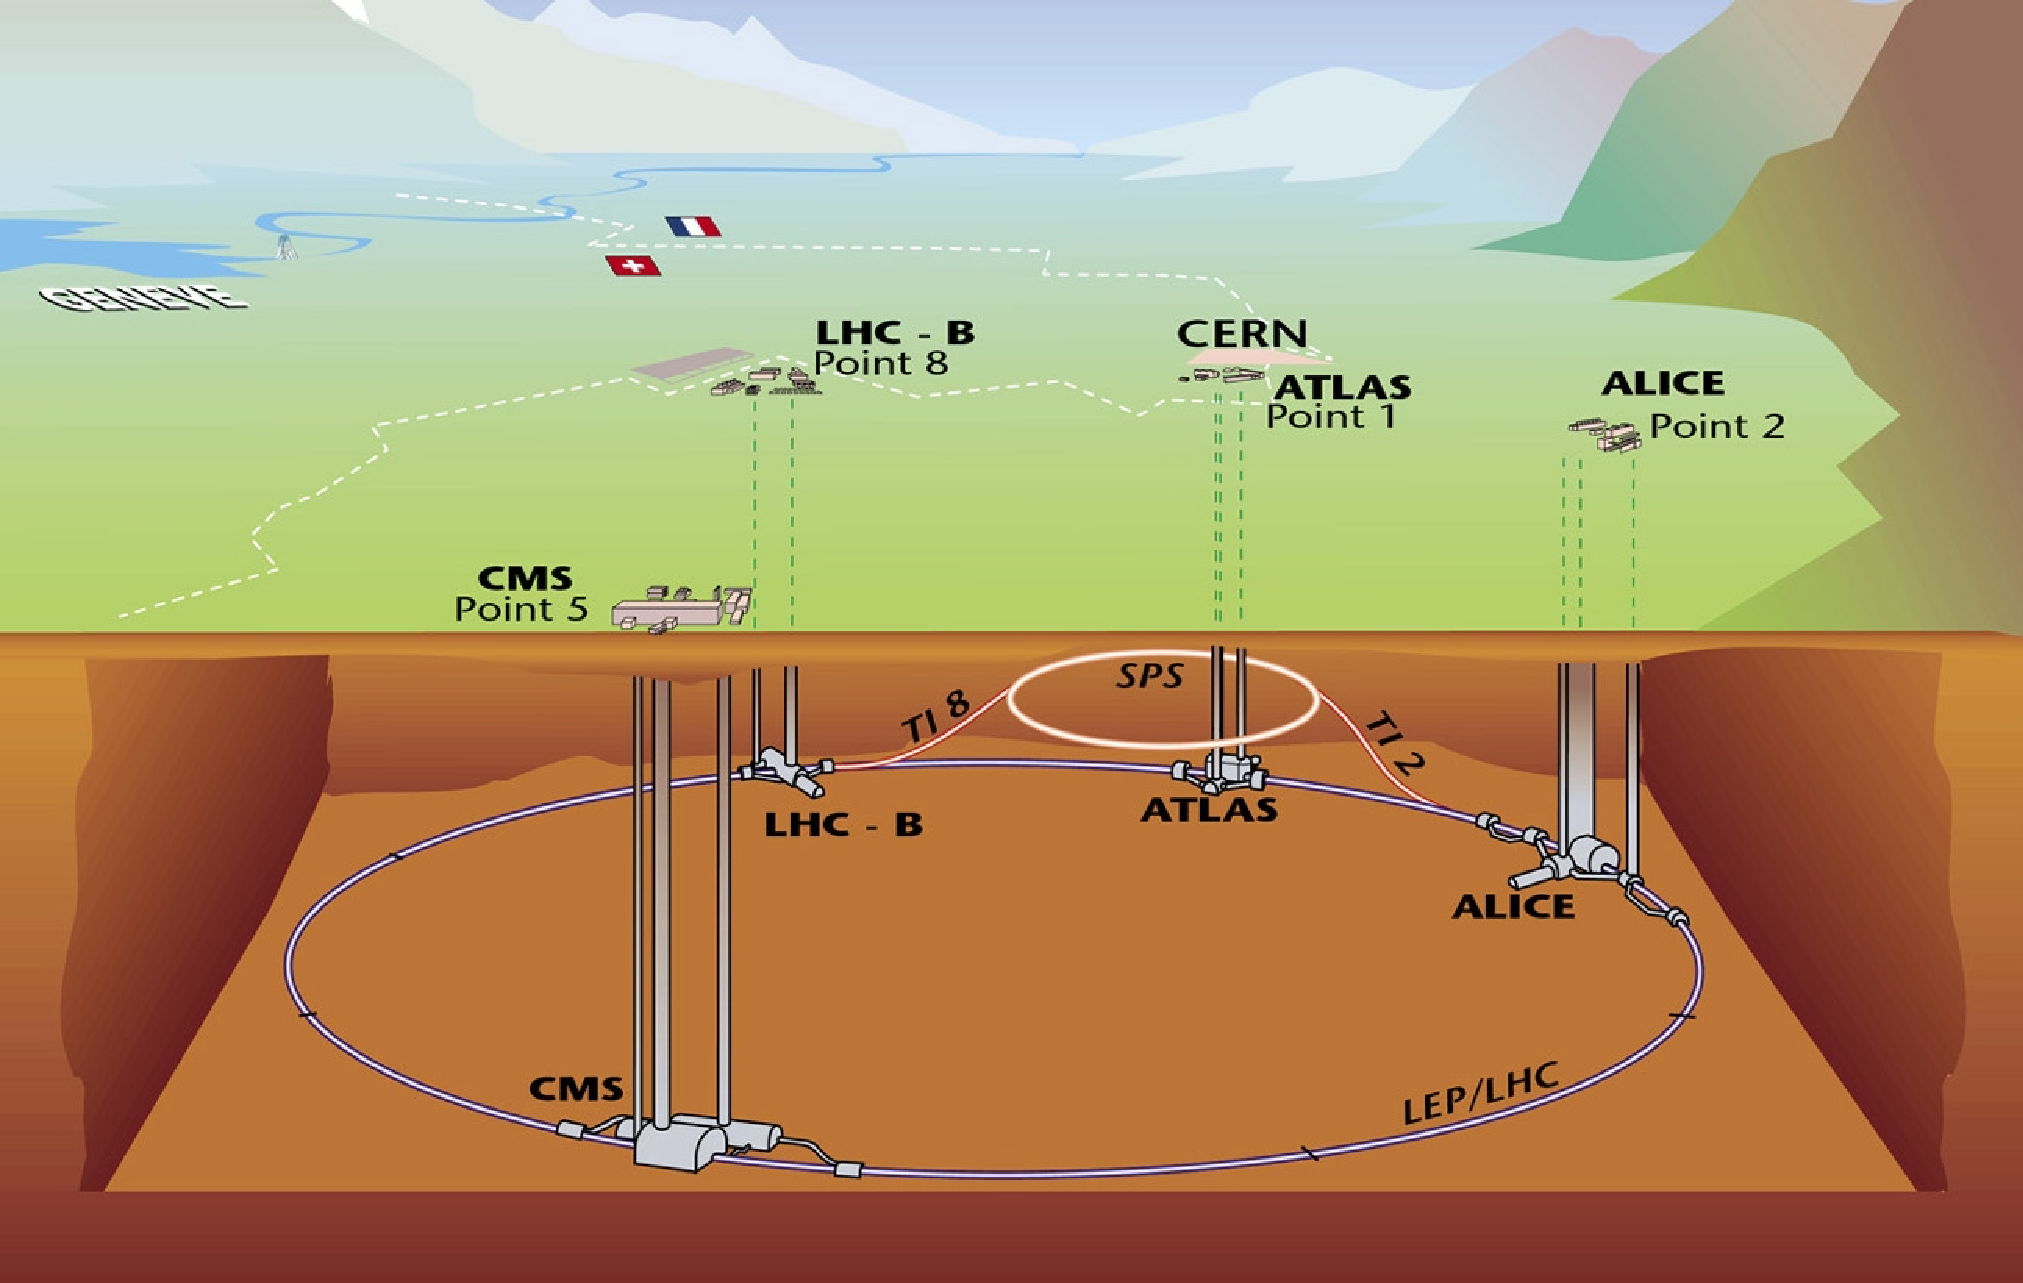
\includegraphics[width=15cm]{cap2_lhc_map2}
\caption{Mapa de localização dos detectores do LHC.} \label{mapaLHC}
\end{figure}
%\cite{Homepage:fotolhc}

%\begin{figure}[h!]
%\centering
%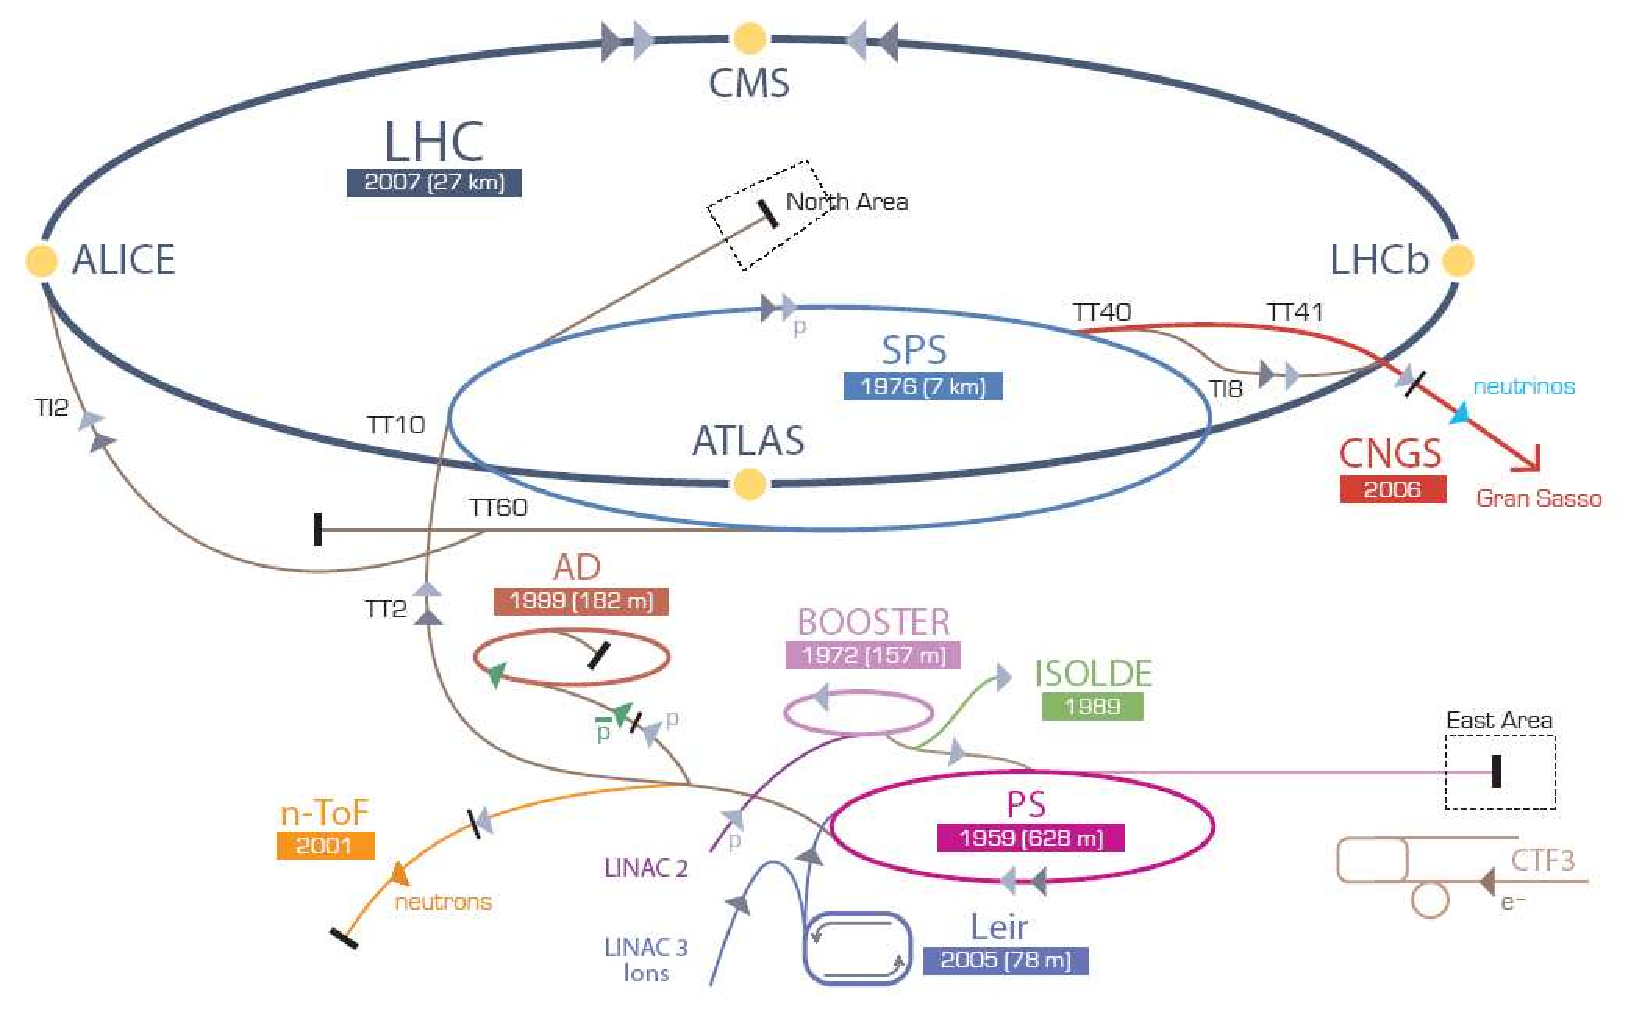
\includegraphics[width=16cm]{cap2_lhc}
%\caption{Diagrama do complexo de aceleradores do CERN com destaque
%para o LHC e seus detectores.} \label{LHC}
%\end{figure}

O LHC tem 6 detectores com propósitos diferentes: ATLAS
\cite{article:ATLAS:2008}, CMS~\cite{article:CMS:2008},
LHCb~\cite{article:LHCb:2008}, LHCf~\cite{article:LHCf:2008}, ALICE
\cite{article:ALICE:2008} e TOTEM \cite{article:TOTEM:2008}. O ATLAS
e o LHCf estão localizados em Meyrin, Suíça, o CMS e o TOTEM em
Cessy, França, o ALICE em St. Genis-Pouilly, França e o LHCb em
Ferney-Voltaire, França (os experimentos TOTEM e LHCf não são
mostrados na Figura \ref{mapaLHC} pois estão em locais próximos respectivamente ao
CMS e ATLAS). O ATLAS (\textit{A Toroidal LHC AparattuS}) e o CMS
(\textit{Compact Muon Solenoid}) são detectores de propósito geral,
enquanto os outros são dedicados a aplicações específicas, como o
LHCb, que é dedicado a explorar informações sobre a física
proveniente dos hádrons do tipo \textbf{b} produzida nas colisões do
LHC.

Quando operando em máxima capacidade, o LHC irá produzir colisões de
feixes de prótons a cada 25 ns e atingirá energia 7 vezes maior que
o Tevatron, que é o acelerador de maior energia em operação
atual\-mente, funcionando no Fermilab.

O número de colisões por centímetro quadrado produzidas por segundo
é chamado de luminosidade (L)~\cite{book:martin:2006}:
\begin{equation}\label{lumi}
    L=n\frac{N_1N_2}{A}f
\end{equation}
onde $n$ é o número de feixes, $N_1$ e $N_2$ o número de partículas
em cada feixe, $A$ a área da seção transversal do feixe e $f$ a
frequência de colisão. Quanto maior a luminosidade do experimento,
maior a quantidade de informação (partículas) gerada.

Quando operando numa luminosidade jamais alcançada ($10^{34}cm^{-2}s^{-1}$), o LHC
deve atingir uma taxa de interações da ordem de 1 GHz. No LHC,
fatores como a alta taxa de interações, as altas doses de radiação,
a multiplicidade de partículas e largas faixas de ener\-gia a cobrir, em conjunto
com a necessidade de medições precisas, definiram novos padrões para
o projeto dos detectores.

A seguir, serão descritas, de modo geral, as principais
características do detector ATLAS.

\section{Características gerais do detector ATLAS}

Os métodos de detecção em física têm como princípio básico promover
interação entre as partículas em estudo e um material conhecido,
produzindo informações sobre a natureza e as características da
própria partícula. Os instrumentos que possibilitam a medição
experimental destas quantidades físicas são chamados de detectores.
Em particular, os detectores de energia são chamados de
calorímetros. À medida que a energia envolvida aumenta, o sistema de
detecção precisa ser mais sofisticado \cite{book:chung:2001}.

O ATLAS foi fruto do trabalho de uma grande colaboração, que envolveu
milhares de físicos, engenheiros, técnicos e estudantes por um
período de vinte anos de projeto, desenvolvimento, fabricação e
instalação.

O detector ATLAS tem 45 m de comprimento, 25 m de altura e pesa aproximadamente
7.000 toneladas, sendo dividido em subsistemas dispostos em camadas.
Conforme ilustrado na Figura \ref{atlas_diag}, os principais
subsistemas são: detector de trajetórias (ou de traço), calorímetros
eletromagnético e hadrônico e os detectores de múons. 

\begin{figure}[h!]
\centering
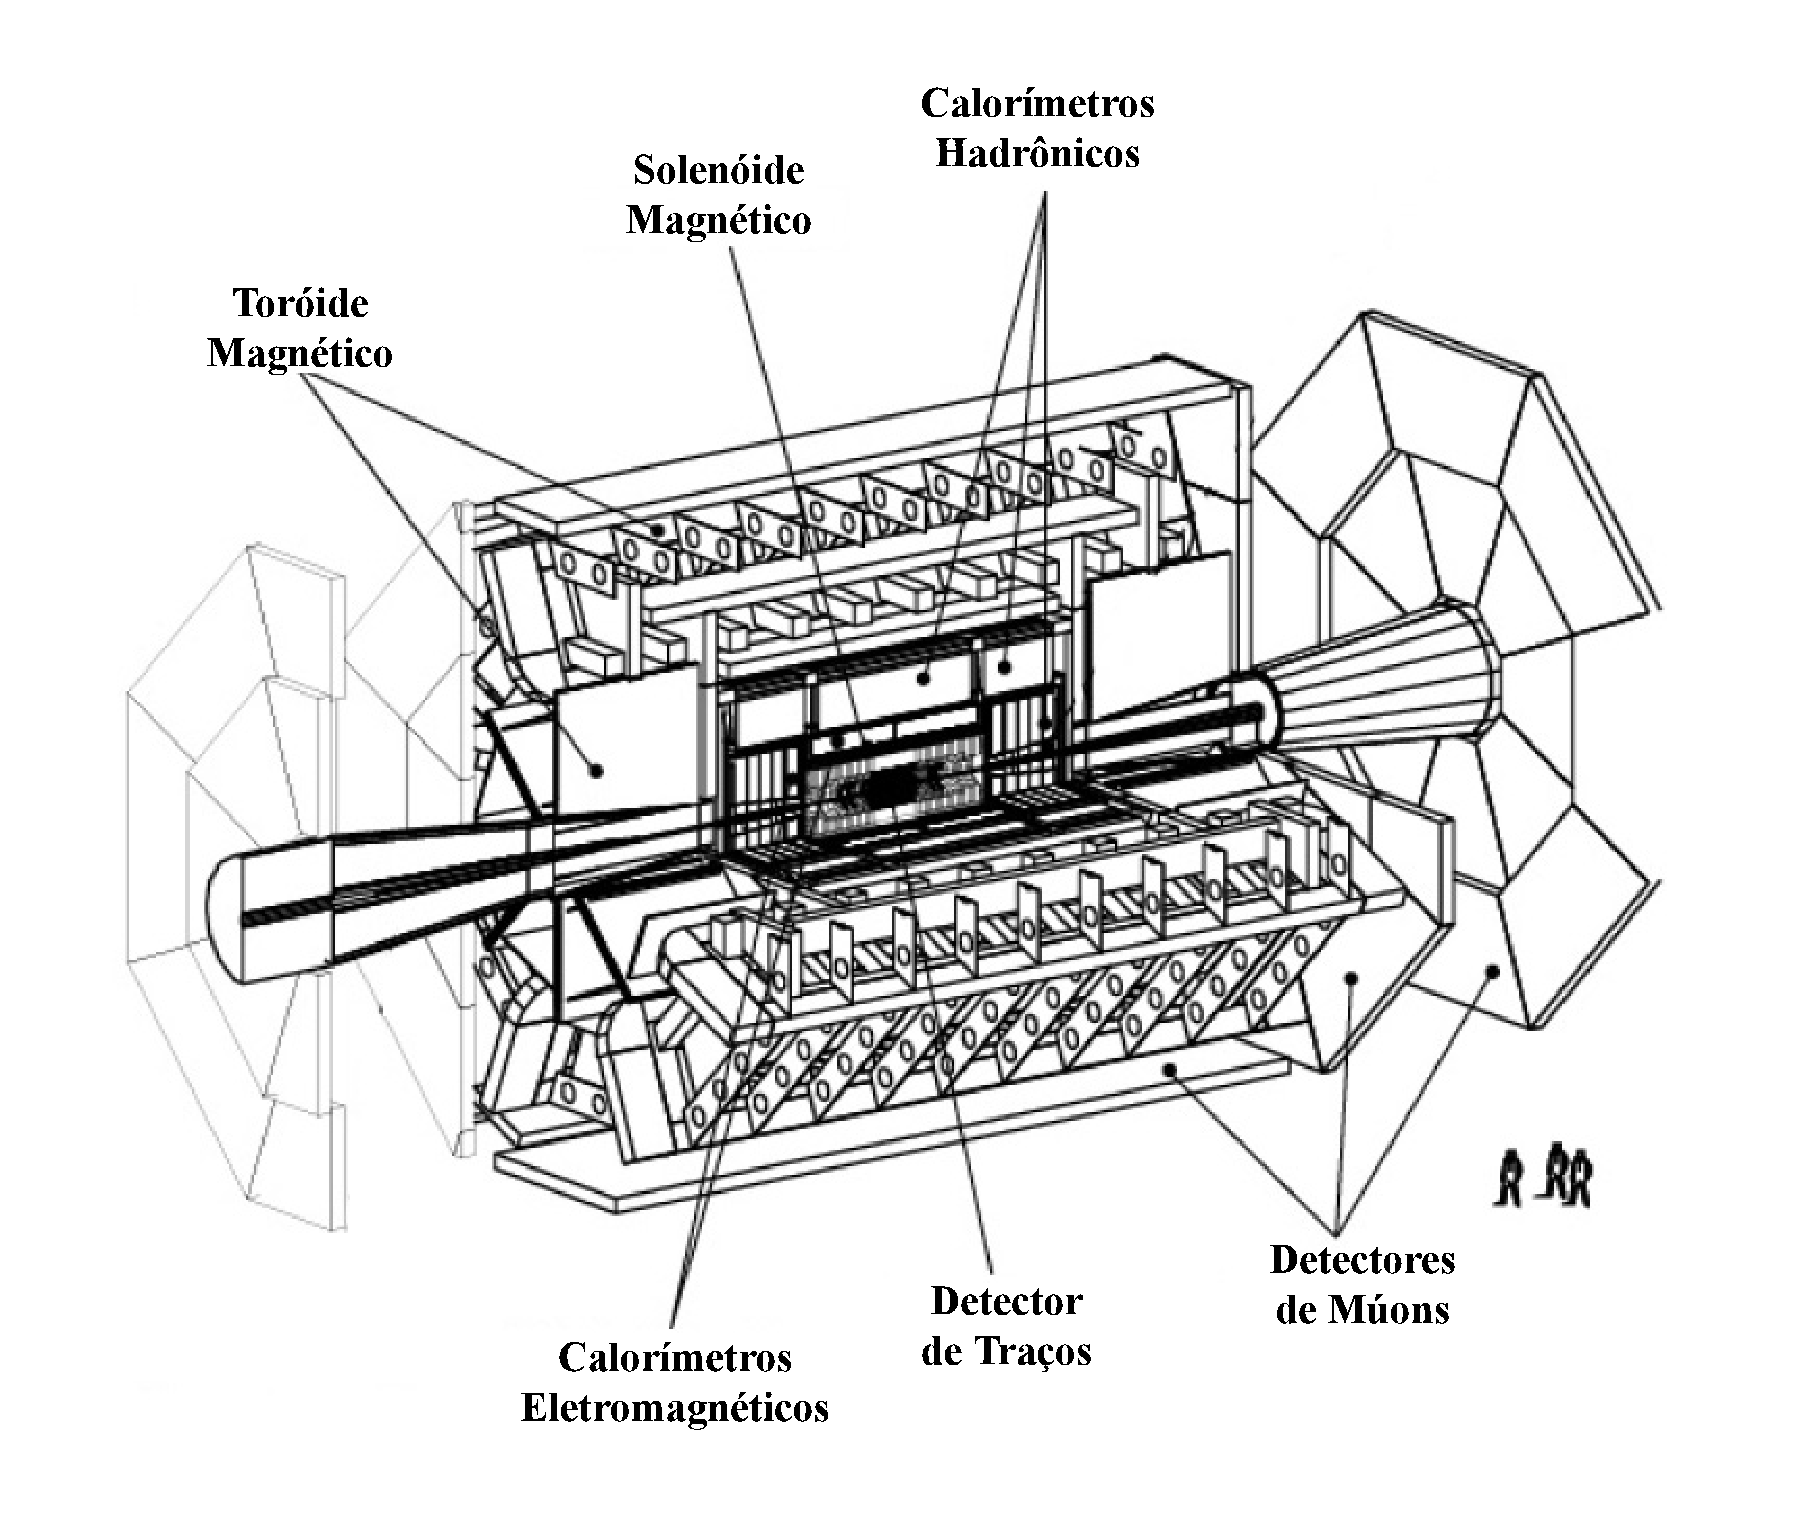
\includegraphics[width=15cm]{cap2_atlas_diag}
\caption{Diagrama esquemático do ATLAS.} \label{atlas_diag}
\end{figure}

A função dos detectores de trajetória é medir o momento das
partículas ele\-tri\-camente carregadas, a partir da curvatura de sua
trajetória, quando imersos no campo magnético do solenóide central \cite{atlastracking:2007}.
Caminhando do eixo central para as extre\-mi\-dades, em sequência,
estão os calorímetros, que medem a energia depositada pelas
partículas \cite{atlascalo:2002}. Na interação com as células do calorímetro, são
produzidos chuveiros de partículas secundárias \cite{book:wigmans:2000}. Num último estágio
está o detector de múons, sistema dedicado à detecção destas partículas, que são as únicas que
não ficam contidas nos calorímetros \cite{atlasmuon:2004}.

O sistema $xyz$ de coordenadas do ATLAS é único para todos os
subsistemas. Conforme mostrado na Figura \ref{atlas_coord}, a
direção do feixe do LHC define o eixo $z$, e os eixos $x$ e $y$
formam um plano transverso ao feixe. A direção positiva do eixo $x$
é definida apontando do ponto de interação para o centro do anel do
LHC, e o eixo $y$ positivo aponta para cima. O ângulo azimutal é
obtido a partir de:

%fazer figura mostrando os angulos ...
\begin{equation}\label{phi}
   \phi=\textrm{arctg}(x/y),
\end{equation}
\\
sendo que $\phi=0$ corresponde ao eixo $x$ positivo e $\phi$ aumenta
no sentido horário. O ângulo polar $\theta$ é medido a partir do
eixo do feixe (eixo $z$ positivo). O momento transverso $p_T$, a
energia transversa $E_T$ e a energia transversa perdida $E_T^{miss}$
são definidas no plano $xy$. A pseudo-rapidez $\eta$ é calculada a
partir do ângulo $\theta$ de es\-pa\-lha\-mento em relação ao eixo
$z$ (ângulo de saída das partículas após a
colisão)~\cite{LI:ATLAS:1992}:

\begin{figure}[b!] \centering
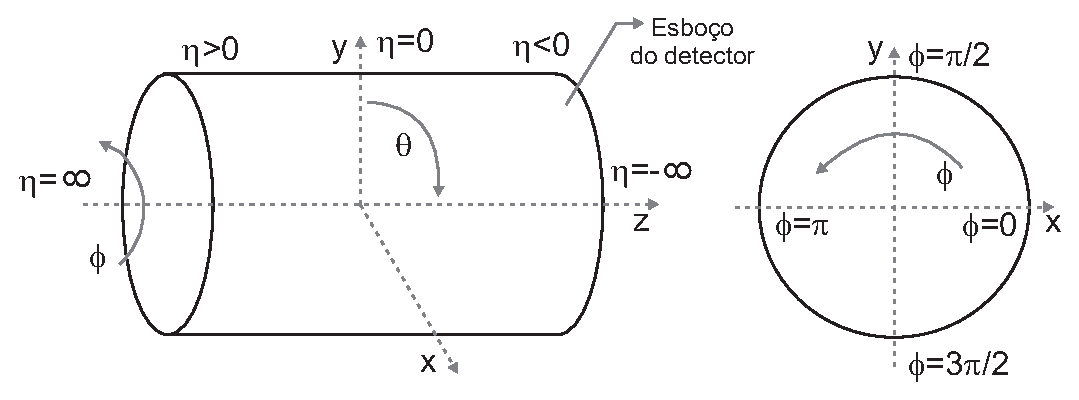
\includegraphics[width=6cm]{cap2_coord}
\caption{Eixo de coordenadas do ATLAS.} \label{atlas_coord}
\end{figure}

\begin{equation}\label{eta}
    \eta=-\ln\textrm{tg}(\theta /2).
\end{equation}
\\
A partir das definições das equações \ref{phi} e \ref{eta},
define-se o eixo ($\eta,\phi$), onde o ângulo $\phi$ representa a
rotação e $\eta$ a direção de projeção das partículas após a
colisão. Grandes valores da pseudo-rapidez indicam que a colisão das
partículas não foi frontal, pois o ângulo de saída, após o choque, é
pequeno, no limite quando $\theta \rightarrow 0$ então $\eta
\rightarrow \infty$. Nesse tipo de colisão, como quase não houve
choque, a produção de partículas elementares é pequena. O ATLAS foi
projetado com baixa resolução para $\eta>3$.

\begin{figure}[tbph]
\begin{center}
\subfigure[]{\label{corte1}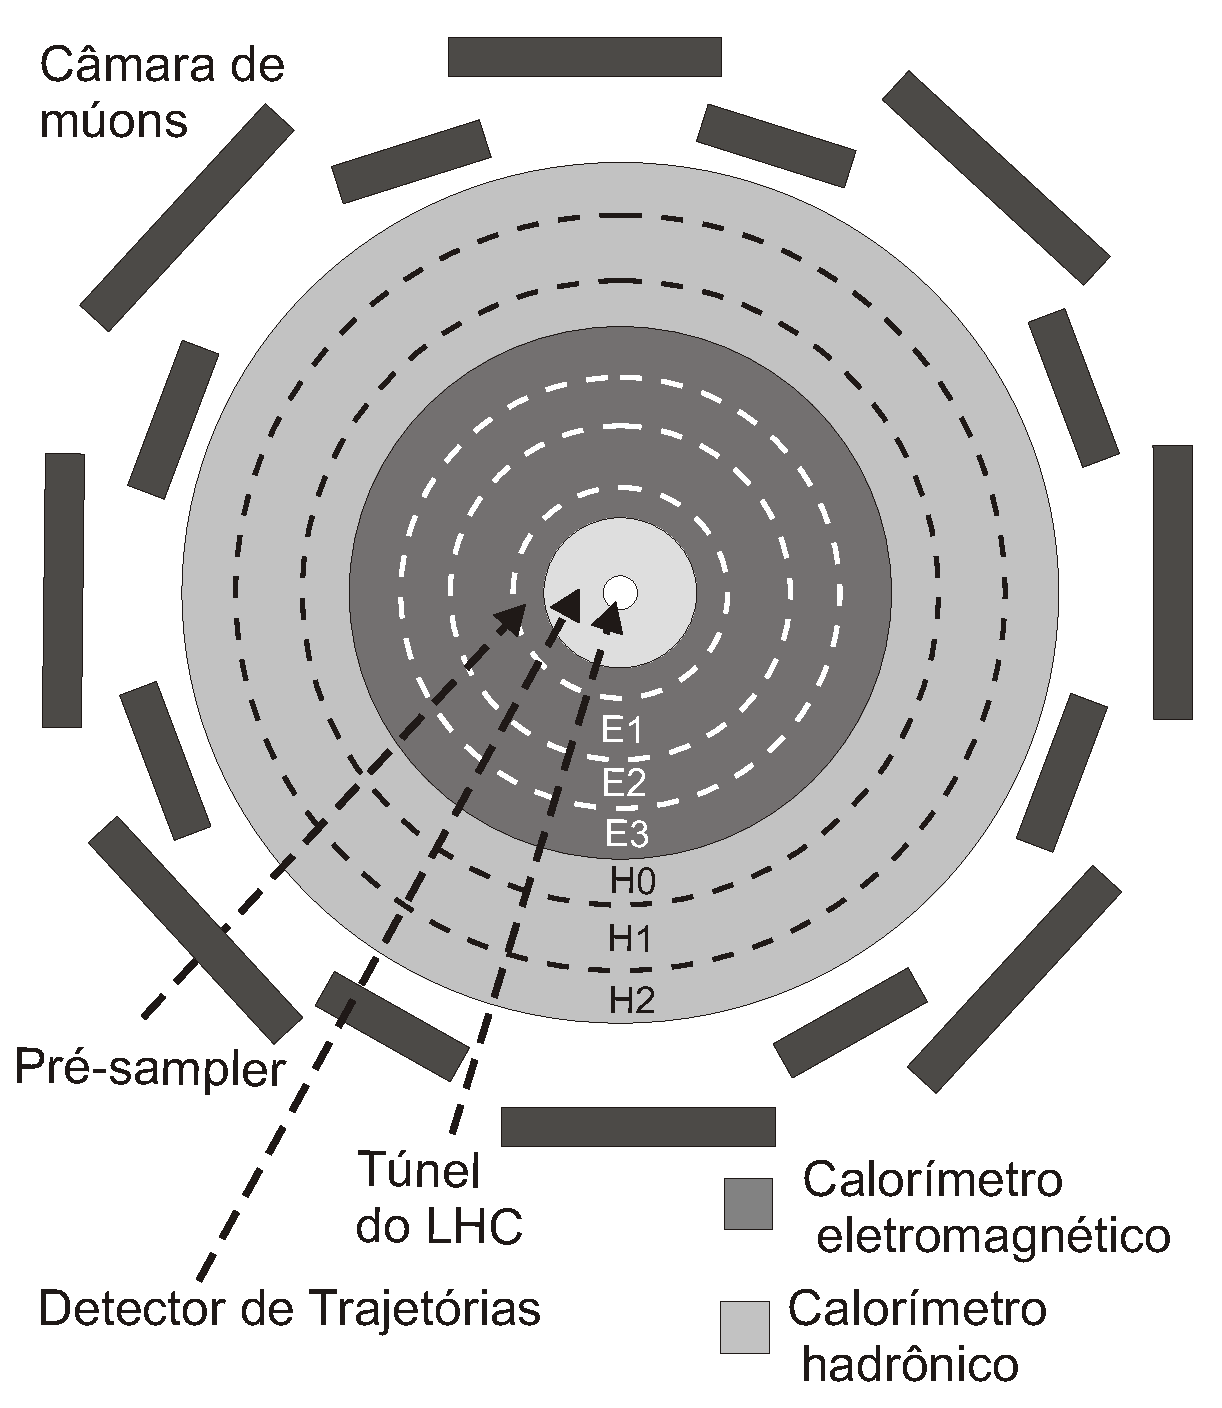
\epsfig{file=cap2_atlas_corte1,width=10cm,clip=}}
\subfigure[]{\label{corte2}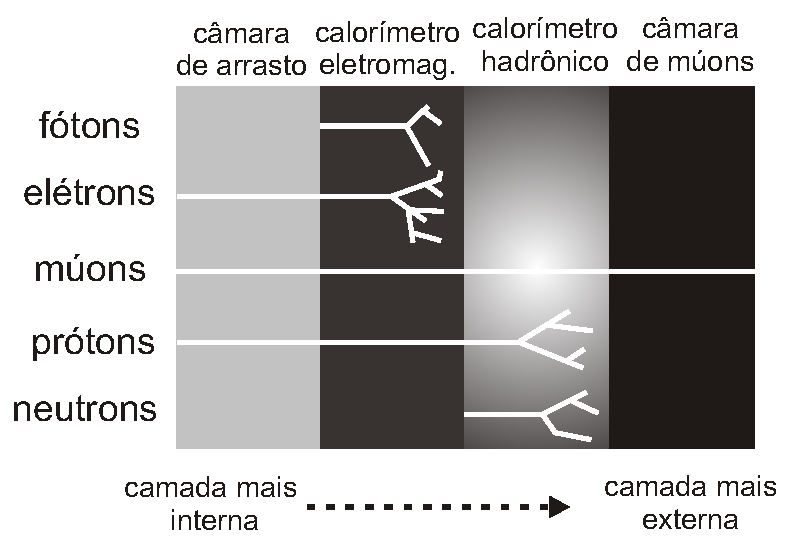
\epsfig{file=cap2_atlas_corte2,width=10cm,clip=}}
\end{center} \caption{Cortes (a) transversal e (b) axial do ATLAS.}
\end{figure}
%, extraídas de \cite{Homepage:ATLAS}

Após uma colisão, as partículas geradas interagem com o material
do detector, perdendo energia e consequentemente velocidade. Na
Figura \ref{corte1} pode-se visualizar os subsistemas do ATLAS num
corte transversal (paralelo ao plano $xy$). Percebe-se que a
câmara de múons e o calorímetro hadrônico têm as maiores
dimensões. Na figura \ref{corte2} é mostrada a penetração e
consequente visualização esperadas de algumas partículas nas
camadas do detector. Não espera-se, por exemplo, deposição de
energia de fótons ou elétrons além das camadas eletromagnéticas do
calorímetro, pois estas partículas interagem intensamente com os
materiais que compõem a seção eletromagnética, perdendo toda sua
energia. As partículas hadrônicas podem interagir com menos intensidade
com o calorímetro eletromagnético e precisam das camadas
hadrônicas para serem paradas. Os múons, em geral, são partículas que
perdem pouca energia nos calorímetros, necessitando de um sistema
especial para serem detectados, o detector de múons.

%parei aqui 24/06

O ATLAS foi projetado e construído considerando-se as condições
experimentais produzidas pelas colisões do LHC e com o objetivo de
obter informações importantes para responder às questões chave em
física de partículas. Entre os principais critérios utilizados para
o projeto do detector pode-se destacar \cite{article:ATLAS:2008}:

\begin{itemize}
  \item Os elementos sensores e circuitos eletrônicos devem
  apresentar resposta rápida e resistência a altos níveis de
  radiação. A fina granularidade do detector é importante para
  reduzir a influência dos eventos sobrepostos.

  \item Excelente calorimetria eletromagnética para a identificação de
elétrons e fótons, complementada por informações acuradas dos
calorímetros hadrônicos, para medições de jatos hadrônicos e energia
transversa $E_T$ (se o valor para $E_T$ for diferente do esperado
isso pode indicar a ocorrência de um fenômeno não observado pelo
detector);

  \item Eficiente sistema de identificação de trajetória para medição do
momento;

  \item Alta precisão na identificação de múons;

  \item Alta aceitação em pseudo-rapidez ($\eta$) com cobertura quase total no
ângulo azimutal ($\phi$);

  \item Alta eficiência do sistema de filtragem (\textit{trigger}),
armazenando a maioria dos eventos físicos de interesse e reduzindo
ao máximo o ruído de fundo (informação não relevante) produzido nas
colisões do LHC.
\end{itemize}

Conforme mencionado no Capítulo 1, o estudo conduzido neste trabalho
utiliza informações do sistema de calorímetros do ATLAS e propõe
algoritmos para a otimização da detecção (trigger) de elétrons. Nas
próximas sub-seções, serão des\-cri\-tos o sistema de calorímetros do
ATLAS e a importância da detecção de elétrons para o desempenho do
experimento.

\subsection{O sistema de calorimetria do ATLAS}

Calorímetros \cite{book:wigmans:2000} representam uma importante classe de
detectores para medição de energia e posição da partícula. Durante o
processo de absorção, as partículas interagem com o material dos
calorímetros gerando partículas secundárias que, por sua vez,
interagem também gerando outras partículas e assim por diante. Este
processo é chamado de cascata ou chuveiro de partículas. Os
calorímetros podem apresentar resposta muito rápida, da ordem de nanosegundos 
\cite{book:wigmans:2000}, e, por isso, é utilizado intensamente pelo sistema
de filtragem online (\textit{trigger}). As prováveis classes de
partículas são identificadas a partir das características esperadas
para o seu perfil de deposição de energia.

Calorímetros são detectores de absorção total. O processo de medição utilizado é destrutivo e as partículas não estão disponíveis após a passagem pelos calorímetros (com excessão aos múons, que conseguem penetrar em grande quantidade de matéria e necessitam de um detector especial a câmara de múons). Quando partículas atravessam matéria, elas em geral interagem e perdem assim uma parte de sua energia. Neste processo o meio é excitado ou aquecido (daí o termo calorimetria). Os calorímetros podem ser classificados em homogêneos ou amostradores. No calorímetro homogêneo todo o volume do detector é sensível às partículas e contribuem para produção do sinal, no calorímetro amostrador o material passivo absorve (interage) as partículas e o material ativo produz o sinal \cite{book:wigmans:2000}.

Partículas como elétrons e pósitrons interagem com a matéria gerando um chuveiro de partículas menos energéticas e necessitam de pequena quantidade de material para serem totalmente absorvidas. Os múons, por outro lado, perdem sua energia muito lentamente necessitando de grande quantidade de matéria para a absorção total. As partículas hadrônicas interagem com a matéria através da força nuclear forte. O processo de interação é muito mais complexo que o EM e uma variedade muito grande de fenômenos pode ocorrer. Os hadrons podem, por exemplo, se comportar de modo semelhante a elétrons e múons, ou se envolverem em uma interação nuclear e se transformarem em 15 novos hádrons. Uma parte da energia das interações hadrônicas não é visível (detectável) pelos calorímetros pois os hadrons neutros não ionizam o calorímetro e a energia é perdida em interações nucleares (fundamentalmente não detectadas pelo calorímetro).

Os calorímetros deveriam ser intrinsecamente lineares para a detecção de partículas EM. Por exemplo um par de elétrons de 10 GeV deveria gerar um sinal de mesma intensidade que um único elétron de 20 GeV. Na prática, desvios do comportamento linear (para partículas EM) podem ser observados na prática devido a fenômenos como:
\begin{itemize}
	\item Saturação das foto-multiplicadoras (PMT – convertem luz dos calorímetros cintiladores em sinais elétricos);
	\item Vazamento do chuveiro: com o aumento da energia algumas partículas podem extrapolar os limites do detector;
	\item Recombinação dos elétrons com íons do material ativo (se isso ocorrem a ionização não é detectada);
	\item Atenuação da luz: a luz emitida pelo material ativo (cintilante) pode ser atenuada antes de atingir as PMT.
\end{itemize}

Calorímetros homogêneos são intrinsecamente não-lineares para a detecção de hadrons e jatos. A fração EM de chuveiros hadrônicos depende da energia e varia bastante de evento para evento, tornando a resposta hadrônica não-constante em função da energia (tanto para calorímetros homogêneos como para os amostradores). A fração não EM (que produz interações nucleares) é, em geral, menor. Em qualquer calorímetro a resolução em energia para hádrons é pior que para elétrons de mesma energia. Isso se deve ao fato de ocorrerem flutuações na energia ``visível” (detectável) aos calorímetros.


Como as características dos chuveiros eletromagnéticos e hadrônicos
são di\-fe\-ren\-tes, na prática, são utilizados tipos de
calorímetro específicos para estas classes de partículas
\cite{book:martin:2006}. O calorímetro eletromagnético é usualmente
instalado internamente ao hadrônico. As partículas eletromagnéticas
(ex: elétrons e fótons) apresentam perfil de deposição de energia
que, em geral, é concentrado em torno do ponto de colisão.
Tipicamente, as partículas eletromagnéticas são absorvidas
completamente nos calorímetros eletromagnéticos. Os chuveiros
hadrônicos apresentam formas va\-ria\-das e iniciam sua interação
com o calorímetro eletromagnético, mas, em geral, somente são completamente
absorvidas nas camadas hadrônicas (mais externas).

O sistema de calorímetros do detector ATLAS
\cite{article:ATLAS:2008} é sub-dividido em 7 camadas \cite{atlascalo:2002}, sendo 4
eletromagnéticas (PS, E1, E2, E3) e 3 hadrônicas (H0, H1 e H2),
conforme Figura \ref{atlas_calo}. Cada camada apresenta diferente
concentração de células detectoras por unidade de área
(granularidade). O calorímetro eletromagnético (EM) é composto de
finas folhas de chumbo separadas por dispositivos sensores de
argônio líquido, cobrindo a região onde $|\eta|<3,2$. As três
camadas do calorímetro eletromagnético são divididas em barril
(região central do detector, onde $|\eta|<1,5$) e tampa (regiões
mais externas onde $1,4<|\eta|<3,2$). Na região onde $|\eta|<1,8$,
imediatamente antes da primeira camada EM existe uma fina camada de
argônio líquido chamada pré-amostrador (\textit{presampler} ou PS).
O pré-amostrador é importante para corrigir medições nas quais
existe perda de energia no caminho até os calorímetros.

Um problema específico do ATLAS é o substancial volume de material ``inerte”(morto) instalado entre o ponto de colisão e os calorímetros. O pré-amostrador tem função primária amenizar os problemas causados pela perda de energia neste material (em 119 GeV ~5\% da energia de elétrons é perdida neste material). Os sinais medidos no PS são ponderados por um fator adequado $\alfa$ e somados aos sinais medidos nas outras camadas para compor a energia total do evento:

\begin{equation}\label{ps}
E_{tot} = E_{calo} + \alfa E_{ps}.
\end{equation}

O calorímetro hadrônico envolve o eletromagnético. Na região
onde $|\eta|<1,7$, ele é composto de placas absorvedoras de aço separadas
por telhas de material plástico cintilante. Quando as partículas
atravessam as telhas elas emitem luz de intensidade proporcional à
energia incidente \cite{TDR1:ATLAS:1999}. O sinal luminoso é então
convertido em elétrico através de placas foto-multiplicadoras. Esta
parte do calorímetro hadrônico do ATLAS é conhecida como calorímetro
de telhas (\textit{Tile Calorimeter} ou simplesmente
\textit{TileCal}) e é dividida em barril ($|\eta|<1,0$) e
barril-extendido ($0,8<|\eta|<1,7$) \cite{article:tilecal:2006}. Para a tampa do calorímetro
hadrônico ($|\eta|>1,5$) utiliza-se a tecnologia do argônio líquido.

\begin{figure}[h]
\centering
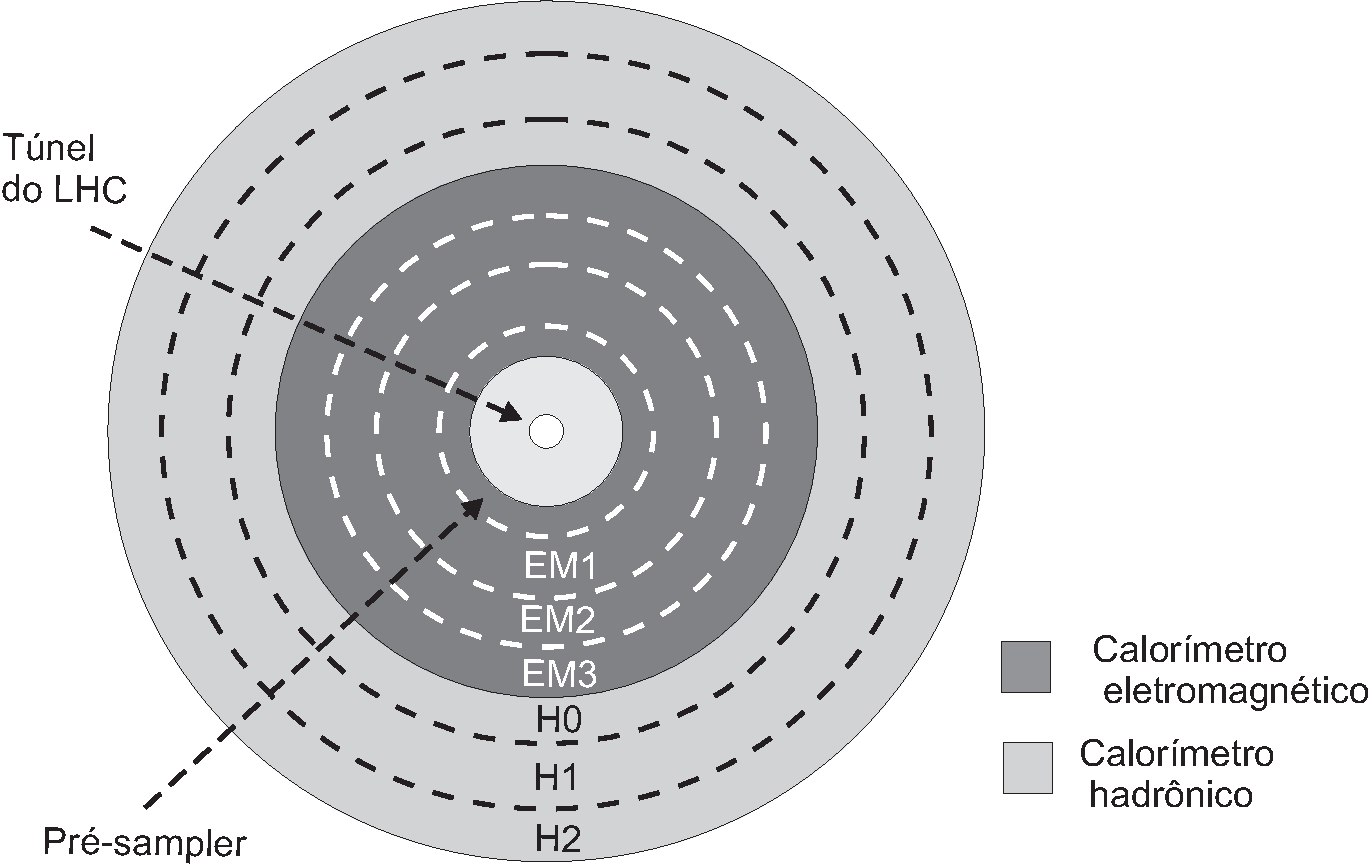
\includegraphics[width=11cm]{cap2_calo}
\caption{Disposição em camadas dos calorímetros do ATLAS.}
\label{atlas_calo}
\end{figure}

A informação da energia depositada nas camadas do calorímetro, com
fina segmentação, é muito importante para a caracterização física
das partículas. Após um evento ser aceito pelo sistema de filtragem,
todas as informações relativas a este evento são armazenadas em
mídia permanente para posterior análise \textit{off-line}. A
granularidade, ou quantidade de células por unidade de área, varia
entre as camadas do calorímetro. A Tabela \ref{tab_calo} traz
informações sobre a região de cobertura em $\eta$, granularidade e
quantidade de canais de leitura (células sensoras) de cada camada do
calorímetro.

\begin{table}[t!]
\centering
\begin{tabular}{l c c}
  \hline
  \hline
  % after \\: \hline or \cline{col1-col2} \cline{col3-col4} ...
  \textbf{Pre-amostrador}    & \textbf{Barril}  & \textbf{Tampa}  \\  \hline
  Cobertura   &  $|\eta|<1,52$ & $1,5<|\eta|<1,8$   \\
  Granularidade ($\Delta \eta \times \Delta \phi$)    &  $0,025 \times 0,1$ & $0,025 \times 0,1$  \\
  Canais de Leitura & 7808 & 1536 (ambos os lados)\\
  \hline
  \hline
  \textbf{Eletromagnético}    & \textbf{Barril}  & \textbf{Tampa}  \\  \hline
  Cobertura   &  $|\eta|<1,475$ & $1,375<|\eta|<3,2$   \\
  Granularidade ($\Delta \eta \times \Delta \phi$)& &  \\
  Camada 1      &  $0,025/8 \times 0,1$ & $0,025/8 \times 0,1$ a $0,1 \times 0,1$  \\
  Camada 2      &  $0,025 \times 0,025$ & $0,025 \times 0,025$ a  $0,1 \times 0,1$  \\
  Camada 3      &  $0,050 \times 0,025$ & $0,05 \times 0,025$   \\
  Canais de Leitura & 101760 & 62208 (ambos os lados)\\
   \hline
   \hline
  \textbf{Had. Telhas Cintilantes}    & \textbf{Barril}  & \textbf{Barril estendido}     \\  \hline
  Cobertura   &  $|\eta|<1,0$ & $0,8<|\eta|<1,7$   \\
  Granularidade ($\Delta \eta \times \Delta \phi$)& &  \\
  Camadas 1, e 2    &  $0,1 \times 0,1$ & $0,1 \times 0,1$   \\
  Camada 3   &  $0,2 \times 0,1$ & $0,2 \times 0,1$   \\
  Canais de Leitura & 5760 & 4092 (ambos os lados)\\
  \hline
     \hline
  \textbf{Had. Argônio Líquido}    & \textbf{Tampa}  &      \\  \hline
  Cobertura   &  $1,5<|\eta|<3,2$  &  \\
  Granularidade ($\Delta \eta \times \Delta \phi$)& &  \\
  Camadas 1, 2 e 3    &  $0,1 \times 0,1$ a $0,2 \times 0,2$ &  \\
  Canais de Leitura & 5632 (ambos os lados)& \\
  \hline
  \hline
\end{tabular}
\caption{Região de cobertura em $\eta$, granularidade e número de
canais de leitura das camadas dos calorímetros.} \label{tab_calo}
\end{table}
%, extraída de \cite{article:ATLAS:2008}

Conforme ilustrado na Figura \ref{calo_cell}, percebe-se que a
primeira camada eletromagnética apresenta mais fina segmentação,
possibilitando medição precisa do ponto de colisão. A segunda camada
apresenta células detectoras quadradas e maior profundidade,
absorvendo maior parcela da energia. A terceira camada, por sua vez,
captura os detalhes do final do chuveiro eletromagnético.

\begin{figure}[h]
\centering
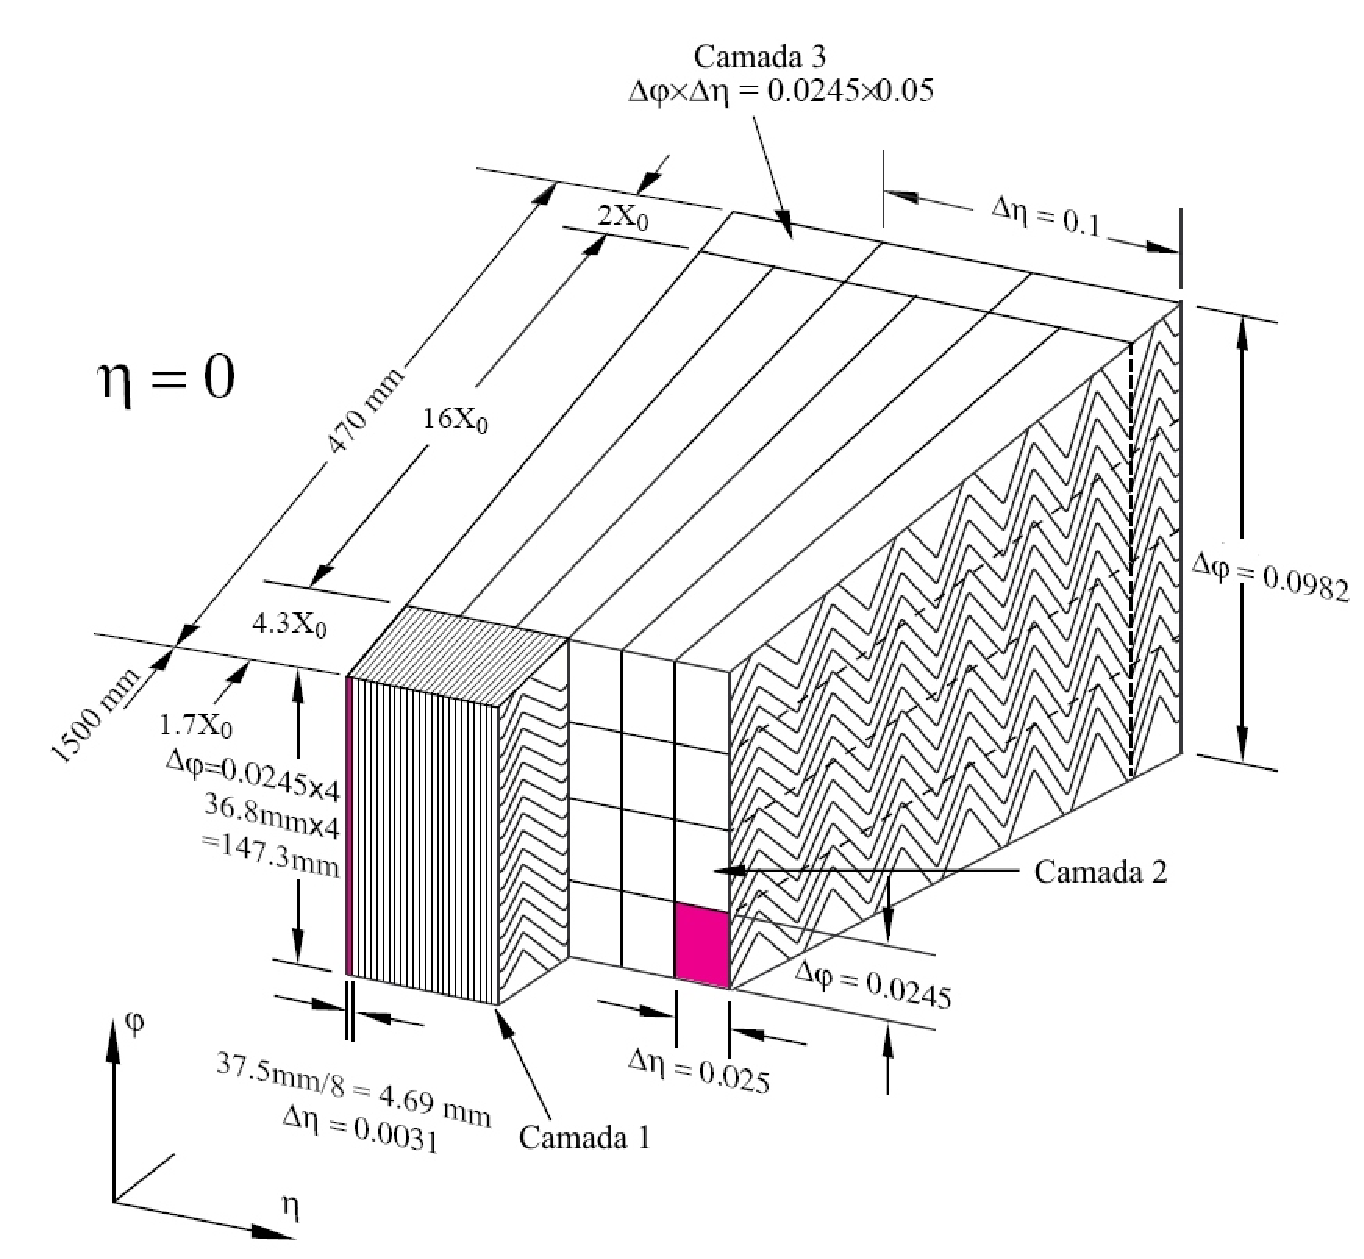
\includegraphics[width=13cm]{cap2_caloem}
\caption{Granularidade e profundidade das camadas do calorímetro
eletromagnético, extraído de \cite{article:ATLAS:2008}.} \label{calo_cell}
\end{figure}
%, adaptada de \cite{article:ATLAS:2008}

Calorímetros são construídos utilizando estruturas modulares. Os cabos de transmissão de sinais e alimentação passam por espaços existentes entre os módulos (\textit{cracks}). No ATLAS, na região de $|\eta|\sim 1,5$ (interconexão entre barril e
barril-extendido) existe uma descontinuidade nos calorímetros
(eletromagnético e hadrônico) para passagem de cabos de alimentação
e dados do detector de trajetória e do barril do calorímetro
eletromagnético \cite{article:ATLAS:2008}. Nesta faixa, há menor
quantidade de células detectoras e, consequentemente, baixa
resolução nas medições obtidas (o que pode representar um problema
para o sistema de filtragem, como será descrito na Seção
\ref{sec_trig}).

Diferente de outros tipos de detectores, a precisão dos calorímetros aumenta com a energia \cite{book:wigmans:2000}:
\begin{equation}\label{res_calo}
    \frac{\sigma_E}{E} \propto \frac{1}{\sqrt{E}}
\end{equation}
onde E é a energia incidente por partícula. Outras fontes de flutuações de menor importância contribuem com fatores de outra ordem como ruído eletrônico: $\propto 1/E$ (domina em baixa energia, principalmente para LAr); e
vazamento lateral do chuveiro: $ \propto 1/(E)^{1/4}$. Uma característica interessante é que as flutuações podem não ser simétricas em torno do valor médio.

Para o calorímetro do ATLAS, foi calculada
experimentalmente em~\cite{atlascalo:2002} a resolução esperada . Os valores encontrados foram $0,1/\sqrt{E}$
e $0,4/\sqrt{E}$, respectivamente para os calorímetros
eletromagnético (de argônio líquido) e hadrônico (de telhas
cintilantes).

Um fato que será freqüente durante o tempo de operação do detector é
a da\-ni\-fi\-cação de células. Devido à alta intensidade de energia
produzida pelas colisões, algumas regiões podem ser danificadas,
deixando de registrar corretamente as informações de energia
depositada, e até parando totalmente de funcionar
\cite{TP:ATLAS:1994}. Os algoritmos de filtragem de eventos devem
ter alguma imunidade à perda de informação das células.

\subsection{Principais objetos de interesse no ATLAS}

Dentre os eventos gerados nas colisões do LHC, apenas uma pequena
parte será útil para a caracterização dos processos da ``nova
física". Com o LHC operando em alta luminosidade podem ocorrer até
10$^9$ interações por segundo, porém, não espera-se mais do que
alguns eventos de interesse por segundo.

Provar a existência do bóson de Higgs é um dos principais objetivos
do LHC. Com o conhecimento adquirido até agora, não é possível
determinar sua massa $m_H$, embora seu limite inferior ($m_H>114$
GeV/c$^2$) tenha sido determinado pelos resultados obtidos em outros
aceleradores, como o LEP (\textit{Large Electron Positron Collider},
acelerador que operou no CERN de 1989 a 2000). O limite superior
esperado por estudos teóricos é $\sim$ 1 TeV/c$^2$
\cite{book:lhc:2008}. Considerando os diversos decaimentos possíveis
para a partícula de Higgs, espera-se que o canal mais limpo para seu
estudo aconteça se sua massa estiver aproximadamente na faixa
150$<m_H<$700 GeV/c$^2$ \cite{article:ATLAS:2008}.

Neste caso, o Higgs pode apresentar o decaimento em 2 bósons Z,
com cada Z, por sua vez, decaindo\footnote{No decaimento de
partículas elementares, parte da massa da partícula é convertida
em energia e o restante em massa de outras partículas} em dois
léptons (elétrons ou múons):
\begin{equation}\label{higgs_dec}
    H \rightarrow ZZ^{(*)} \rightarrow l^+ l^- l^+ l^-
\end{equation}

Para este canal de busca do Higgs, é fundamental que os detectores
tenham um sistema de filtragem capaz de identificar com alta
eficiência elétrons e múons. Estas duas partículas, assim como os
fótons, jatos e os taus, são importantes também para o melhor
entendimento da supersimetria (SUSY - \emph{supersimetry})
\cite{livro:fisica1:2006}. Os taus também podem levar aos modelos
de Higgs estendidos \cite{TDR2:ATLAS:1999}. Um resumo com os
principais objetos de interesse no ATLAS e suas aplicações na
física pode ser encontrado na Tabela \ref{tab_fisica}.

\begin{table}[h!]
\centering
\begin{tabular}{c c }
  \hline
  % after \\: \hline or \cline{col1-col2} \cline{col3-col4} ...
  \textbf{Objeto}    & \textbf{Física de interesse}       \\  \hline
  \textbf{Elétron}   &  Higgs, SUSY, dimensões-extra, novos bósons e \textit{top quark}\\
  \textbf{Fóton}    &  Higgs, SUSY e dimensões-extra\\
  \textbf{Múon}      & Higgs, SUSY, extra-dimensões, novos bósons e \textit{top quark}\\
  \textbf{Jato}   &  SUSY e ressonâncias\\
  \textbf{Jato + $E_T^{miss}$}    &SUSY e \textit{leptoquarks}\\
  \textbf{Tau + $E_T^{miss}$}      & Modelo de Higgs estendido e SUSY\\
  \hline
\end{tabular}
\caption{Principais objetos de interesse no ATLAS.}
\label{tab_fisica}
\end{table}
%, extraída de \cite{article:HLT1:2003}

A identificação destes objetos dentro de um universo enorme de
informações é realizada pelo sistema de filtragem
(\textit{trigger}). Conforme mencionado, um dos objetos de
interesse na filtragem do ATLAS é o elétron. Para a identificação
de elétrons, a informação obtida no sistema de calorímetros é
muito importante. Em termos da calorimetria, as assinaturas de
elétrons podem ser confundidas com perfis de energia gerados por
alguns jatos hadrônicos (espacialmente concentradas nas camadas
eletromegnéticas e com pouca energia nas hadrônicas). Considerando
que a produção de jatos será muito frequente nas colisões do LHC,
estes formarão um intenso ruído de fundo para a identificação de
elétrons. Pelo que foi exposto, percebe-se que a discriminação
elétron/jato (e$^-$/j) é importante para o desempenho do detector.


\section{O sistema \textit{online} de filtragem do ATLAS}
\label{sec_trig}

Quando operando em alta luminosidade ($10^{34}cm^{-2}s^{-1}$) o
LHC deve atingir uma taxa de interações de 1 GHz. Entretanto, a
freqüência de ocorrência de eventos de interesse para a física
pode ser muito pequena. Espera-se que, por exemplo, se os bósons
de Higgs existirem, conforme previstos no Modelo Padrão, eles
ocorram com freqüência inferior a 0,001 Hz \cite{TDR:ATLAS:1998}.
As estratégias de aceitação de eventos devem garantir que as
informações de interesse não sejam perdidas, reduzindo ao máximo a
quantidade de eventos não relevantes gravados em mídia permanente.

Considerando que, a cada evento (colisão) no ATLAS são gerados
aproximadamente 1,5 MByte de informação e que o LHC produz uma
colisão a cada 25ns, ou seja uma taxa de $40\times 10^6$ eventos por
segundo, chega-se então a aproximadamente 60 TBytes de informação
por segundo. Com a tecnologia disponível atualmente não é possível
armazenar essa quantidade de informação. Mesmo que fosse viável
acumular as leituras de todos os eventos, o processo de filtragem
\textit{offline} seria extremamente demorado. Assim, é necessário um
sistema eficiente de filtragem \textit{online}.

O sistema de filtragem do ATLAS (usualmente chamado de sistema de
\textit{trigger}) acessa informação dos três principais
sub-detectores, o detector de trajetórias, os calorímetros e a
câmara de múons. O \textit{trigger} online opera em 3 níveis
seqüenciais de seleção de eventos, o nível 1 (LVL1), o nível 2
(LVL2) e o filtro de eventos (EV - \textit{event filter}), sendo que
os dois últimos compõem a filtragem de alto nível (HLT -
\textit{High Level Trigger}). Cada nível é responsável pela rejeição
de uma parcela das assinaturas não relevantes e refina a decisão do
nível anterior. A Figura \ref{trigger} ilustra as principais
características dos três níveis de filtragem de eventos no ATLAS.

\begin{figure}[h!] \centering
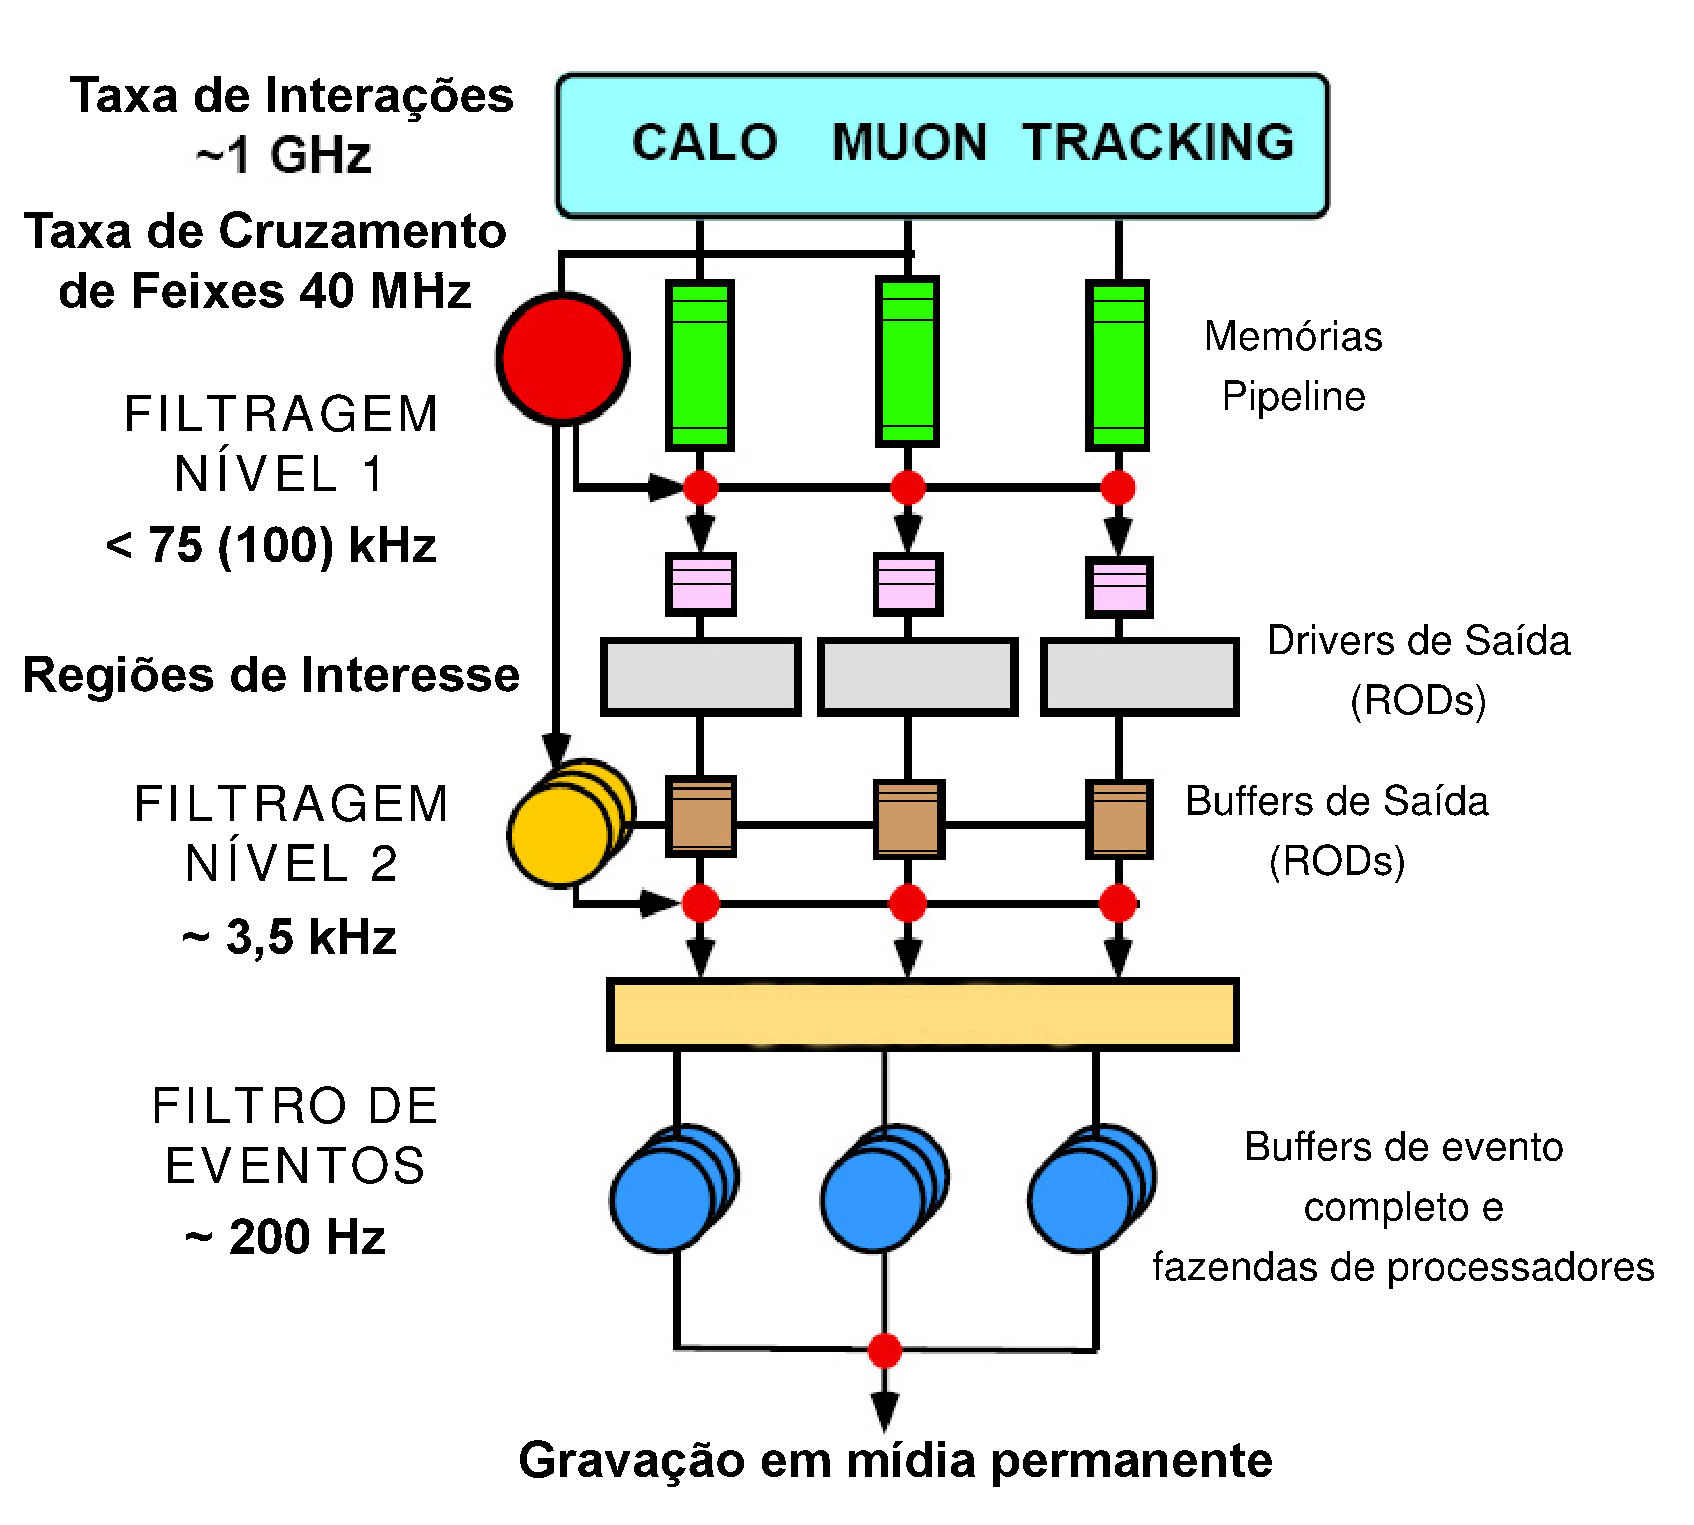
\includegraphics[width=13cm]{cap2_trigger}
\caption{Diagrama em blocos do sistema de filtragem e aquisição de
dados do ATLAS.} \label{trigger}
\end{figure}
%, extraído de \cite{TDR1:ATLAS:1999}

O primeiro nível tem sérias restrições quanto ao tempo de
processamento (latência de 2,5$\mu s$), recebendo a plena taxa de
eventos do LHC como entrada. Esse nível é implementado em
\textit{hardware} dedicado, usando apenas parte da re\-so\-lução
disponível ao detector. O LVL1 entrega ao segundo nível a
localização das áreas onde possivelmente aconteceram eventos de
interesse, regiões estas conhecidas como RoI (\textit{Regions of
Interest}). A seleção de eventos no LVL2 é feita através de
\textit{software} especializado, rodando em um conjunto de 1500 PCs
dedicados operando em paralelo. Neste nível, o tempo máximo para
tomada de decisão é 40 ms e informações do detector de trajetórias,
assim como a total resolução dos calorímetros, estão disponíveis. A
seleção de eventos do HLT deve fazer uso otimizado dos recursos de
CPU e rede disponíveis. Isso motiva o projeto das estratégias de
extração de características utilizando o processamento em regiões de
interesse (RoIs), e o processo de validação passo a passo (ver
Figura \ref{trigger}). Para os calorímetros, as RoIs típicas têm
dimensões de $0,4 \times 0,4$ no plano $\eta \times \phi$. O filtro
de eventos é o último estágio do sistema de filtragem, recebendo uma
taxa de eventos mais baixa, tendo assim latência de alguns segundos
para tomada de decisão. A estratégia de processamento seqüencial
permite que os eventos sejam rejeitados na primeira etapa possível,
minimizando a necessidade de acesso a informações, e facilitando o
ajuste e eventual modificação das estratégias de extração de
características. Na Tabela \ref{tab_trigg} é apresentado um resumo
das principais características dos 3 níveis de filtragem do ATLAS.

\begin{table}[h!]
\centering
\begin{tabular}{c c c c c c}
  \hline
  % after \\: \hline or \cline{col1-col2} \cline{col3-col4} ...
  \textbf{Nível} & \textbf{Te (Hz)}       & \textbf{Ts (Hz)}      & \textbf{Cr}    & \textbf{Latência (s)} & \textbf{Implementação}\\  \hline
  \textbf{LVL1}   &  $40\times10^6$        & $75\times (100) 10^3$ &  533 (400)  & 2,5$ \times 10^{-6}$  & \textit{Hardware}\\
  \textbf{LVL2}   &  $75 (100)\times  10^3$ & $3,5\times10^3$         & 21 (29)      & $40 \times 10^{-3}$   & \textit{Software} \\
  \textbf{EF}     & $3,5\times10^3$          & $\approx 200 $                   & 17            & $\approx 4$           & \textit{Software}\\
  \hline
\end{tabular}
\caption{Principais características do sistema de \textit{trigger}
do ATLAS, onde $Te$ e $Ts$ são, respectivamente, as taxas de eventos
na entrada e na saída e $Cr=Te/Ts$ é o coeficiente de redução de
eventos.} \label{tab_trigg}
\end{table}

Um problema que afetará os algoritmos de extração de
características é o efeito de empilhamento (do inglês
\textit{pile-up}), que ocorre quando há uma sobreposição de
eventos em regiões do detector \cite{article:seixas:1996}, ou
seja, um evento que ainda se desenvolve tem seu padrão de
deposição de energia distorcido por um novo evento que chega e se
sobrepõe, gerando um ruído de fundo que pode atingir grande
intensidade.

Para o projeto e teste dos métodos de extração de características,
foram usados conhecimentos prévios adquiridos em outras experiências
com aceleradores de partículas e eventos simulados através de
técnicas de Monte Carlo \cite{book:montecarlo:2004}. As
si\-mu\-la\-ções utilizam modelos estocásticos que descrevem as interações,
 levando em conta as carac\-terísticas físicas do
acelerador e do detector, assim como os efeitos de cada nível de
filtragem. Para o ATLAS, foram utilizados ge\-ra\-do\-res de eventos
para colisões próton-próton como HERWIG, ISAJET e PYTHIA, descritos
em \cite{TDR1:ATLAS:1999} e \cite{TDR:ATLAS:2003}. Os algoritmos de
classificação e extração de carac\-terísticas foram projetados para
os dados simulados e serão posteriormente adaptados para a realidade
de operação quando do início da aquisição de dados.

\subsection{Primeiro nível de filtragem}

Conforme mostrado na Figura \ref{trigger} e na Tabela
\ref{tab_trigg}, o primeiro nível de filtragem é responsável por
reduzir a taxa de eventos de aproximadamente 40 MHz para 75 kHz (a
taxa de saída do LVL1 pode ser aumentada até 100 kHz a depender
das condições de operação do detector). A decisão do primeiro
nível deve ser tomada até $2,5\mu s$ após o cruzamento de feixes
(colisão) ao qual o evento está associado.

%Com estas restrições o LVL1 está sendo implementado utilizando
%\textit{hardware} dedicado, através de dispositivos lógicos
%programáveis de alto desempenho como CPLDs (\textit{Complex
%Programmable Logic Device}) e FPGAs (\textit{Field-Programmable Gate
%Array}).

O LVL1 identifica as assinaturas básicas de interesse e, para tornar
mais rápida a tomada de decisão, a granularidade dos subsistemas do
detector é reduzida \cite{TDR:ATLAS:1998}. Considerando o sistema de
calorímetros, que possui mais de 100.000 células detectoras, o LVL1
utiliza apenas 7000 torres de soma analógicas (as torres são obtidas
somando-se a energia de células dentro de regiões de 0,1$\times$0,1
em $\Delta\eta \times \Delta\phi$). Até a tomada de decisão de nível
1 toda a informação do detector é armazenada em memórias tipo
\textit{pipeline}. Quando um evento é aceito, as informações
referentes são descarregadas para uso pelo nível 2 de filtragem. As
informações dos eventos não aceitos são descartadas neste ponto.

A tomada de decisão quanto à aceitação ou rejeição de eventos no
nível 1 é feita pelo processador central de \textit{trigger}
(\textit{central trigger processor} - CTP), que combina as
informações disponíveis nos calorímetros e na câmara de múons,
conforme mostrado na Figura \ref{lvl1}, e possibilita o uso de
diferentes menus de filtragem.

\begin{figure} \centering
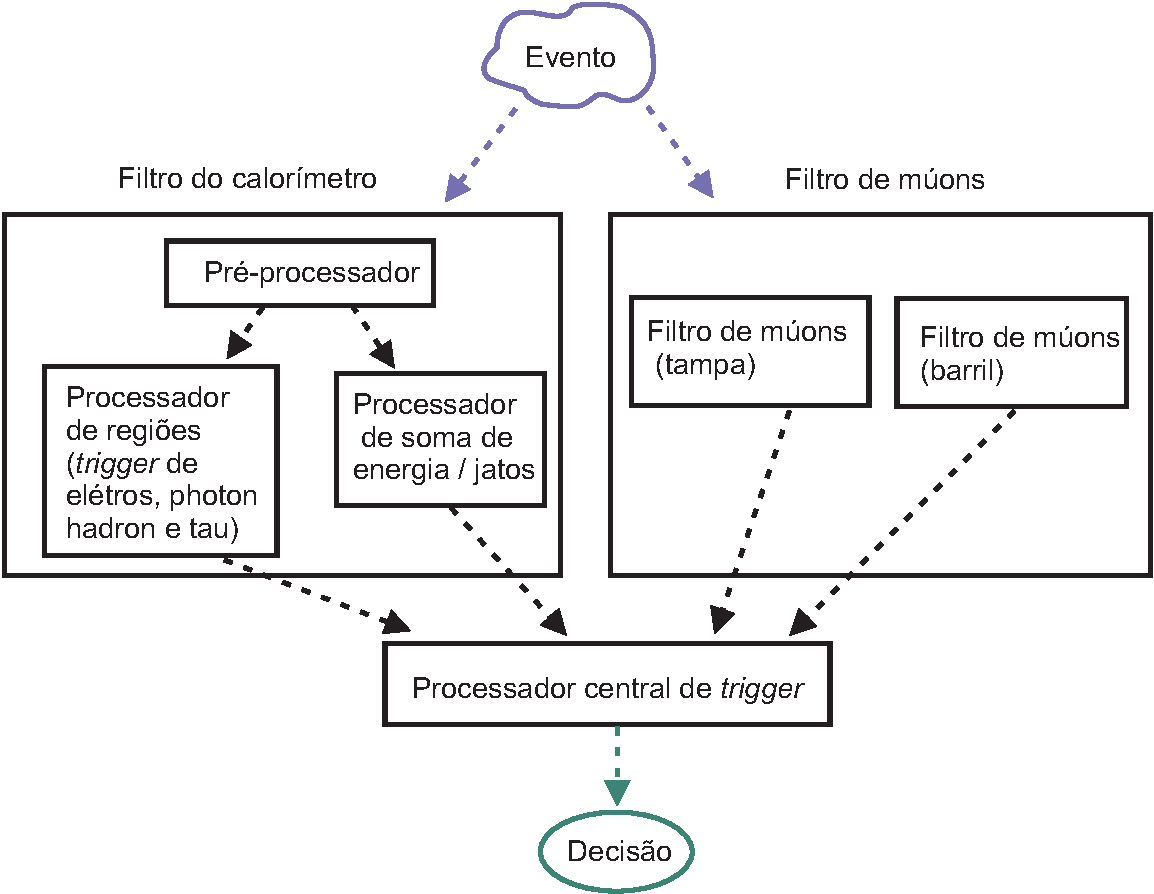
\includegraphics[width=13cm]{cap2_nivel1}
\caption{Diagrama em blocos do primeiro nível de filtragem.}
\label{lvl1}
\end{figure}
%, adaptado de \cite{TDR:ATLAS:1998}

O primeiro nível fornece para o nível 2 informações sobre as
regiões de inte\-resse (RoI). As RoI sinalizam as áreas que
precisam ser analisadas nos níveis mais altos de filtragem. O
nível 1 também fornece outras informações importantes, como o
critério utilizado para aceitação do evento, as componentes do
vetor $E_T^{miss}$ e a posição no plano ($\eta$,$\phi$). O nível 2
tem acesso, se necessário, a toda a informação do evento com total
precisão e granularidade, mas em geral apenas uma pequena parte
destes dados é utilizada.

Na Tabela \ref{tab_lvl1} são mostradas as freqüências dos
principais canais de filtragem esperadas para o LVL1 quando o LHC
estiver operando em alta luminosidade (L=10$^{34}$cm$^{-2}s{-1}$).
Pode-se perceber que a taxa total simulada é da ordem de 40 kHz,
aproximadamente 2 vezes menor que a freqüência de saída esperada
para o nível 1 que pode chegar a 100 kHz. Isso se deve às
incertezas nos cálculos realizados a partir dos eventos simulados
\cite{TDR:ATLAS:1998}.

\begin{table}
\centering
\begin{tabular}{c c}
  \hline
  % after \\: \hline or \cline{col1-col2} \cline{col3-col4} ...
  \textbf{Canal} & \textbf{Freqüência (kHz)} \\  \hline
  Um múon  &  4 \\
  Par de múons  & 1 \\
  Região eletromagnética & 22 \\
  Par de regiões eletromagnéticas & 5 \\
  Um jato & 0,2 \\
  Três jatos & 0,2 \\
  Quatro jatos & 0,2 \\
  Jato e $E_T^{miss}$ & 0,5 \\
  Tau e $E_T^{miss}$ & 1 \\
  Múon e região eletromagnética & 0,4 \\
  Outras condições & 5 \\ \hline
  \textbf{Total} & \textbf{$\approx$ 40} \\
  \hline
\end{tabular}
\caption{Freqüência esperada para os principais canais de
\textit{trigger} no primeiro nível de filtragem do ATLAS
(L=10$^{34}$cm$^{-2}s{-1}$).} \label{tab_lvl1}
\end{table}
%, extraída de \cite{TDR:ATLAS:1998}

\subsubsection{Filtragem de elétrons no LVL1}

A filtragem de elétrons no LVL1 é baseada em cortes lineares em
parâmetros do perfil de deposição de energia medido nos
calorímetros. A definição dos critérios de seleção leva em conta o
conhecimento das características típicas do perfil de deposição de
energia de objetos eletromagnéticos (elétrons e fótons), que
tipicamente apresentam:
\begin{itemize}
  \item concentração ao redor do ponto de colisão;
  \item alta concentração de energia na seção eletromagnética;
  \item pouca ou nenhuma energia na seção hadrônica.
\end{itemize}

Conforme dito anteriormente, no primeiro nível de filtragem as
células dos calorímetros são somadas para formar sinais conhecidos
como torres de \textit{trigger} (TT). Cada TT cobre uma área de 0,1
$\times$ 0,1 no plano $\eta \times \phi$ no calorímetro
eletromagnético e 0,2 $\times$ 0,2 no hadrônico. A partir da análise
de uma janela deslizante cobrindo uma região de 4 $\times$ 4 TT (16
no total), quatro critérios podem ser utilizados pelo LVL1 para
definir um possível candidato a elétron, são eles:
\begin{enumerate}
  \item Haver mais energia na região central de 2 $\times$ 2 TT, do
  que na periferia;
  \item As energias das TTs da região central (de 2 $\times$ 2 TT)
  são somadas duas a duas e utiliza-se o maior valor encontrado, que deve exceder um patamar de energia eletromagnética;
  \item O nível de energia na periferia (fora da região central de 2 $\times$ 2
  TT) é calculado para verificar o isolamento em energia do objeto
  em questão;
  \item A energia nas camadas hadrônicas é somada para verificar o
  vazamento de energia fora do calorímetro eletromagnético (isolamento hadrônico).
\end{enumerate}
Os patamares de seleção do nível 1 podem ser ajustados e os
critérios combinados a depender das características da física de
interesse que se deseja estudar num dado momento de operação do
detector.

\begin{figure} \centering
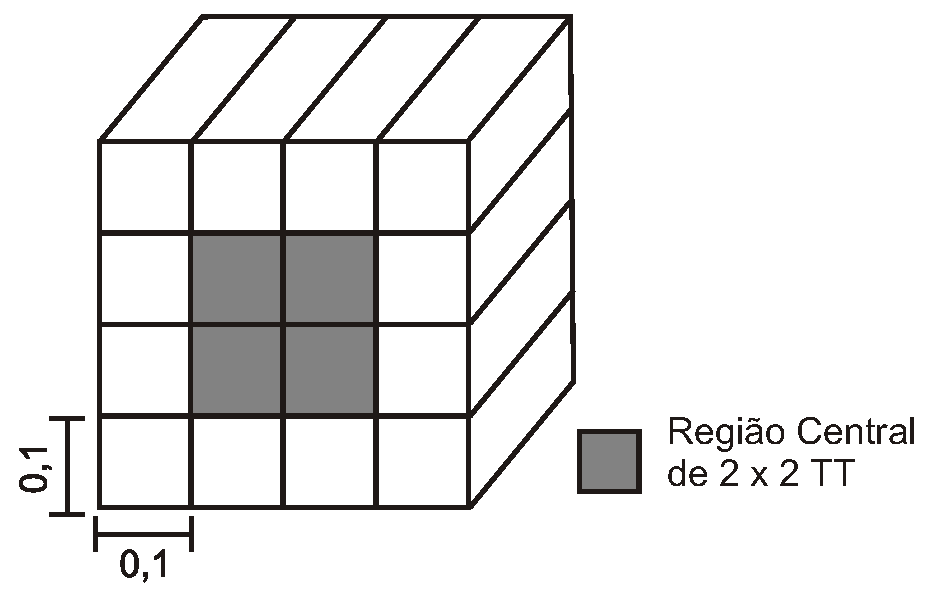
\includegraphics[width=9cm]{cap2_trigger_tower}
\caption{Janela deslizante analisada pelo LVL1 no calorímetro
eletromagnético.} \label{lvl1}
\end{figure}

\subsection{Filtragem de alto nível}

O sistema de filtragem de nível 2 (LVL2) e o filtro de eventos (EF)
são responsáveis pela filtragem de alto nível (HLT -
\textit{high-level trigger}) do ATLAS. O nível 2 deve reduzir a taxa
de eventos de 75 kHz (podendo chegar até 100 kHz) para 3,5 kHz,
tendo um tempo de latência de aproximadamente 40 ms para tomar a
decisão \cite{TDR:ATLAS:2003}. O EF precisa diminuir a taxa de
eventos de 3,5 kHz para 200 Hz. Os eventos que forem aceitos pelos
três níveis de filtragem serão armazenados em mídia permanente para
futura análise \textit{offline}. O tempo para a tomada de decisão no
filtro de eventos é de alguns segundos. O HLT é implementado em
\textit{software} e opera em um conjunto de PCs em paralelo. Embora
existam algoritmos desenvolvidos pela colaboração do ATLAS para a
filtragem de alto nível (nos diversos canais de interesse),
pesquisas continuam sendo conduzidas com o objetivo de propor
rotinas de filtragem alternativas que forneçam maior eficiência de
discriminação da física de interesse e, ao mesmo tempo, maior
rejeição do ruído de fundo.

Considerando os efeitos conjuntos do segundo nível e do filtro de
eventos, a filtragem de alto nível deve reduzir em aproximadamente
500 vezes a taxa de eventos. As etapas de processamento do HLT são
iniciadas pelo acesso às informações das RoI, fornecidas pelo
LVL1. A extração de características é efetuada em cada sistema do
detector, iniciando pela confirmação da RoI no sistema onde esta
foi originada (câmara de múons ou calorímetro), seguida pela
confirmação em outros sistemas, como a câmara de arrasto
\cite{TDR1:ATLAS:1999}. Os principais objetos de \textit{trigger}
identificados no HLT são candidatos a múons, elétrons, fótons,
taus, jatos, $E_T^{miss}$ e física dos hádrons b. As informações
necessárias para a decisão do alto nível dependem do tipo de
região de interesse fornecida pelo LVL1, cada uma tendo suas
próprias características de processamento \cite{TDR:ATLAS:2003}. O
desempenho geral é medido a partir da eficiência na discriminação
da física de interesse e do ruído de fundo. As principais
características desejadas para os algoritmos de filtragem no LVL2
são listadas a seguir:

%, extraídos de \cite{TDR:ATLAS:2003}

\begin{itemize}
  \item alta eficiência ($>$ 95\%) por RoI selecionada no LVL1;

  \item eficiência uniforme em $\eta$ e eficiência uniforme ou
  crescente com $E_T$;

  \item redução do ruído de fundo minimizando a taxa de eventos classificados de forma incorreta (falso
  alarme);

  \item robustez em relação à luminosidade, ruído de medição, imperfeições de ali\-nha\-men\-to e calibração.

\end{itemize}

Um diagrama de blocos do sistema de filtragem de alto nível é
mostrado na Figura~\ref{lvl2}. As informações dos sub-detectores
(calorímetros, câmaras de arrasto e de múons) são utilizadas
inicialmente pelo nível 1, enquanto isso, são armazenadas em
memórias temporárias, para posterior uso pelo nível 2. O acesso aos
dados dos sub-detectores pelo \textit{trigger} de alto nível é feito
através dos \textit{Read Out Buffers} (ROB). As informações das RoI
são armazenadas nos RoIB (\textit{Region of Interest Buffers}). Mais
informações sobre os componentes dos sistemas de filtragem podem ser
encontradas em \cite{TDR:ATLAS:1998}, \cite{TDR:ATLAS:2003},
\cite{TDR1:ATLAS:1999} e \cite{TDR2:ATLAS:1999}.

%detalhar mais o sistema de trigger aqui

Conforme mencionado anteriormente, a filtragem de alto nível pode
utilizar toda a granularidade e precisão dos subdetectores do ATLAS.
Então, percebe-se que, os algoritmos do HLT operam num espaço de
decisão multidimensional, com restrições no tempo de processamento e
rígidos padrões de eficiência. Deve-se notar também que, as
características do sistema de filtragem podem mudar com o melhor
conhe\-ci\-men\-to do detector, após os testes e o início de
operação. Percebe-se, então, que o sistema de \textit{trigger} de
alto nível demanda esforços no sentido de propor, testar e comparar
diferentes estratégias de seleção.

\begin{figure}[t!]
\centering
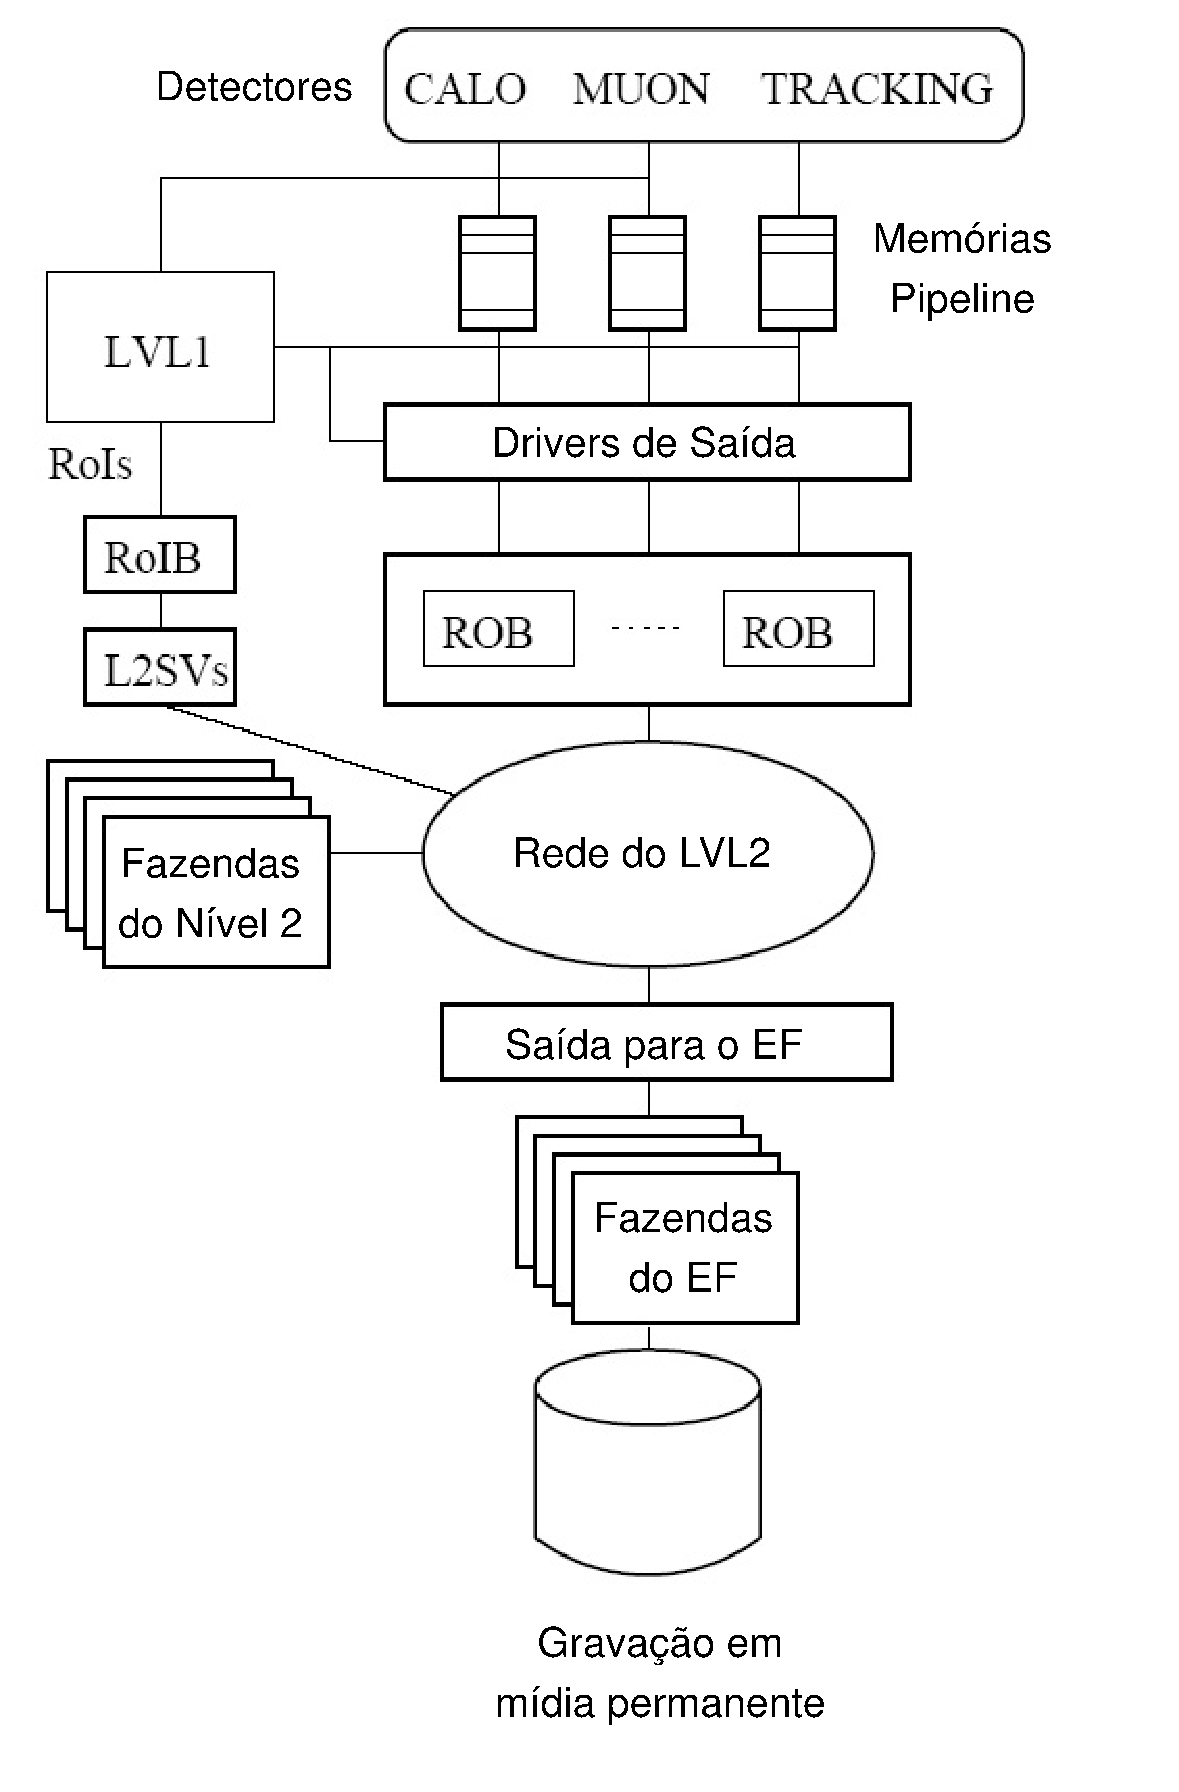
\includegraphics[width=9.5cm]{cap2_nivel2}
\caption{Diagrama em blocos do segundo nível de filtragem.}
\label{lvl2}
\end{figure}

%parei aqui em 17/07/09 %%%%%%%%%%%%%%%%%%%

\subsubsection{Filtragem de elétrons no LVL2}

%falar do calo

O \textbf{T2Calo} \cite{TDR:ATLAS:2003} é o algoritmo padrão para
extração de características e teste de hipóteses adotado no
segundo nível de filtragem do ATLAS. Esse algoritmo utiliza
informações de calorimetria, sendo capaz de separar objetos
eletromagnéticos isolados de jatos hadrô\-nicos, utilizando
parâmetros que estimam a forma dos chuveiros de deposição de
energia \cite{TDR:ATLAS:2003}.

O primeiro passo do T2Calo é refinar a posição da RoI fornecida pelo
LVL1, encontrando a célula de maior energia na segunda camada do
calorímetro eletromagnético. Essa posição ($\eta_1 , \phi_1$) será
posteriormente refinada pelo cálculo da posição da média ponderada
da energia em uma janela de $3 \times 7$ em ($\eta , \phi$). Para a
seleção dos objetos eletromagnéticos são calculados os parâmetros:
\begin{itemize}
  \item $R_{\eta}^{shape}=E_{37}/E_{77}$, onde $E_{nm}$ é a energia
  depositada numa janela de $n \times m$ em torno de ($\eta_1 ,
  \phi_1$);

  \item $R_{\eta}^{strip}=(E_{1st}-E_{2nd})/(E_{1st}+E_{2nd})$ é
  obtida em uma janela de $\Delta \eta \times \Delta \phi=0,125 \times
  0,2$, onde $E_{1st}$ e $E_{2nd}$ são o máximo e o segundo maior
  valor de energia encontrados depois de somar em $\phi$ para cada posição
  $\eta$;

  \item A energia total $E$ depositada no calorímetro
  eletromagnético é calculada em uma janela de $3 \times 7$ células
  em torno de ($\eta_1 ,   \phi_1$);

  \item A energia que passa para o calorímetro hadrônico $E^{had}$ é
  calculada em uma janela de $\Delta \eta \times \Delta \phi=0,2 \times
  0,2$ em torno do novo centro da RoI calculado pelo T2Calo.

\end{itemize}

%\subsubsection{T2 Hypo}

Considerando que o perfil de deposição de energia dos elétrons é,
em geral, mais concentrado ao redor do ponto de máximo e que,
também não espera-se deposição de uma quantidade significativa de
energia nas camadas hadrônicas por elétrons, percebe-se que, o
T2Calo opera através de cortes lineares utilizando informações da
física de interesse.

Técnicas de extração de características e classificação que fazem
uso do processamento estatístico de sinais e cortes não-lineares no
espaço de busca foram propostas como uma alternativa ao T2Calo para
a discriminação elétron/jato no LVL2. Exem\-plos podem ser
encontrados em \cite{article:anjos:2006} e
\cite{article:herman:2006}.

Como resultado destes trabalhos, foi implementado na plataforma de
software do ATLAS o discriminador Neural-Ringer
\cite{article:anjos:2006,tese:andre:2006}, que utiliza um
classificador neural supervisionado para o canal elétron-jato no
LVL2. Para extração de características, os sinais dos calorímetros
são formatados em anéis concêntricos de deposição de energia (mais
detalhes a respeito serão fornecidos no Capítulo 4). Este
discriminador apresentou desempenho superior ao T2Calo, com tempo de
processamento que, embora seja maior, atende aos requisitos do nível
2.

Num ambiente complexo como o que é gerado a cada colisão do LHC,
onde o nível de ruído de fundo é extremamente alto e os eventos de
interesse são raros, qualquer melhora na eficiência dos algoritmos
de filtragem significa menor quantidade de eventos não relevantes
armazenados mídia permanente, facilitando a análise
\textit{offline}.

O sucesso obtido com o Neural-Ringer motiva a busca por técnicas de
pré-processamento que contribuam para a otimização do custo
computacional, ou para o aumento da eficiência de discriminação.
Neste contexto, o presente trabalho propõe o uso de técnicas de
extração de características como Análise de Componentes
Independentes e métodos correlatos para a compactação da informação
e extração de características discriminantes. No próximo capítulo,
as técnicas de aprendizado estatístico para extração de
características e classificação utilizadas neste trabalho serão
descritas e comentadas.
